\documentclass[hidelinks,a4paper, 10pt, nofootinbib]{article}

\usepackage[width=15.5cm, left=3cm, top=2.5cm, right=2cm, left=2cm, height= 24.5cm]{geometry}
\usepackage[spanish, es-tabla]{babel} %es-tabla es para que ponga Tabla en vez de Cuadro en el caption
\usepackage[utf8]{inputenc}
\usepackage[T1]{fontenc}
\usepackage{xspace}
\usepackage{xargs}
\usepackage{fancyhdr}
\usepackage{lastpage}
\usepackage{caratula}
\usepackage[bottom]{footmisc}
\usepackage{amsmath}
\usepackage{amssymb}

\usepackage{float}% http://ctan.org/pkg/float

\usepackage{algorithm}
\usepackage[noend]{algpseudocode}
\usepackage{array}
\usepackage{xcolor,colortbl}
\usepackage{amsthm}
\usepackage{listings}
\usepackage{svg}

\usepackage{pgf}
\usepackage{tikz}
\usetikzlibrary{arrows,automata}

\usepackage{graphicx}
\usepackage{sidecap}
\usepackage{amsmath}
\usepackage{wrapfig}

\usepackage{caption}
\captionsetup[figure]{labelformat=empty}% redefines the caption setup of the figures environment in the beamer class.

\usepackage{hyperref}
\hypersetup{
  colorlinks   = true, %Colours links instead of ugly boxes
  urlcolor     = blue, %Colour for external hyperlinks
  linkcolor    = blue, %Colour of internal links
  citecolor   = red %Colour of citations
}

\usepackage{comment}

\usepackage[
  backend=bibtex,
  style=alphabetic
]{biblatex}
\addbibresource{bibliografia.bib}


\captionsetup[table]{labelsep=space}


\setlength{\parindent}{1em}
\setlength{\parskip}{0em}

%Defino colores para las tablas
\definecolor{LightCyan}{rgb}{0.77,0.9,0.9}
\definecolor{Gray}{gray}{0.8}
\definecolor{azul}{HTML}{0040C0}
\definecolor{rojo}{HTML}{FD0A10}



%%fancyhdr
\pagestyle{fancy}
\thispagestyle{fancy}
\addtolength{\headheight}{1pt}
\lhead{Algoritmos y Estructuras de Datos 3 - TP3}
\rhead{$1^{er}$ cuatrimestre - 2017}
\cfoot{\thepage\ / \pageref{LastPage}}
\renewcommand{\footrulewidth}{0.4pt}
\renewcommand{\labelitemi}{$\bullet$}

%%caratula
\materia{Algoritmos y Estructuras de Datos III}
\titulo{Trabajo Práctico 3}
%\subtitulo{}
%\grupo{Grupo 12}
\integrante{Seijo, Jonathan Adrián}{592/15}{jon.seijo@gmail.com}
\integrante{Reyes Mesarra, Darío René}{838/15}{eran6reyes@gmail.com}
\integrante{Cordoba, Lucas}{094/15}{lmcordobaa@gmail.com}
\integrante{Balbachan, Alexis}{994/12}{alexisbalbachan@gmail.com}

\fecha{Junio 2017}

\usepackage{etoolbox}
\AtBeginEnvironment{tikzpicture}{\shorthandoff{>}\shorthandoff{<}}{}{}

\usepackage[draft]{todonotes}

\begin{document}

\maketitle
\tableofcontents

\newpage
% !TEX root = ./informe.tex

\section{Motivación}

Un \textit{clique} en un grafo $G$ es un subconjunto de vértices que induce en $G$ un subgrafo completo. La \textit{frontera} de un subconjunto de vértices $S$ es el conjunto de vértices con un extremo en $S$ y otro en $G \setminus S$. El presente informe analiza el problema de encontrar un clique que maximice la cardinalidad de su frontera en un grafo determinado. Dicho problema pertenece a la clase $NP$, por lo que es un problema dificil de resolver, y será de interés qué calidad de respuestas podemos conseguir en un tiempo razonable. \\

Antes de embarcarnos en esta aventura (lol), veamos por qué calcular el clique con máxima frontera de un grafo es un problema interesante con posibles aplicaciones reales. Primero hablaremos un poco de qué puede llegar a modelar un `clique', y que información de este puede darnos su frontera. \\

La palabra `clique' proviene de la sociologia, en donde representa un grupo unido de individuos con intereses en común. Modelando redes sociales con grafos, la definición formal de clique que acabamos de realizar hasta cierto punto coincide con esta noción. Esto ocurre porque el hecho de que un grupo de personas en una red induzca un subgrafo completo implica que todas las personas están conectadas entre sí. Esto nos da la pauta de que podríamos calcular `cliques' para conocer mejor las dinámicas dentro de una red social. También pueden utilizarse en el contexto de la química, por ejemplo, para detectar similaridades estructurales entre proteinas distintas \cite{proteins}. Pensando en el complemento de un grafo, también pueden ayudarnos a encontrar conjuntos de vértices independientes. \\

Orientados al problema CMF, el caso de las redes sociales es de particular interés. Mencionamos que un `clique' puede representar un grupo cohesivo de personas. Una observación razonable es que adyacencia total dos a dos puede ser una condicción demasiado restrictiva para caracterizar a un grupo en un modelo estándar de relaciones personales. Sin embargo, hay formas de sortear estos problemas, como utilizar la definición de \textit{n-cliques} (Luce 1950, Alba 1973), que grosso modo, es una estrategia para relajar las adyacencias dentro de un grafo. El objetivo es admitir grupos como n-cliques que no calificarian estrictamente como cliques. De cualquier forma, lo que queremos transmitir es que generalmente es posible asumir que la definición clique se corresponde bien con los grupos en redes sociales modeladas como grafos. \\

Lidiando con redes sociales con mucha información, podemos utilizar los cliques para presentar la información de forma más compacta y más representativa, lidiando con grupos en vez de individuos. \\

\vspace{-1cm}
\begin{center}
	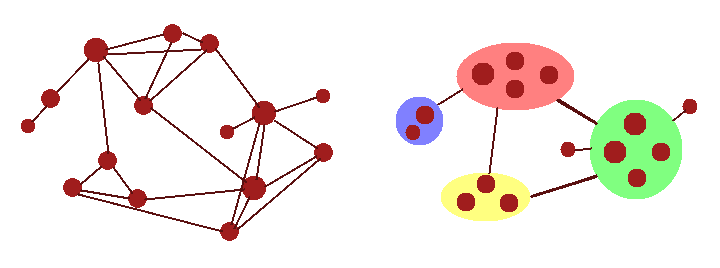
\includegraphics[scale=0.9]{informe/imgs/example.png}
	\textit{A la izquierda un grafo que modela una pequeña hipotética red social. A la derecha representamos la misma red social agrupando los individuos mediante cliques disjuntos maximales. En esta última imagen, los ejes entre cliques representan la existencia de elementos en ambos conjuntos que están conectados entre sí.}
\end{center}

Vemos como esto puede permitirnos identificar mejor las dinámicas grupales. Además, parece apropiado analizar redes sociales en torno a los grupos dentro de la misma, ya que son una unidad más representativa en términos del impacto que tienen en la red. \\

Al pensar en cliques representativos de una red, una idea sencilla es buscar los cliques más grandes, maximizando la cantidad de vértices. No es la única forma, y aquí es justamente donde entra la definición de frontera. ¿Qué representa una frontera para un clique? Por definición, son todas las conexiones que `cruzan' el clique, esto es, que conectan algún miembro del clique con alguién de afuera. Si medimos qué tan conocido es un individuo por la cantidad de amigos que tiene, entonces tiene sentido medir qué tan conocido es un clique por la cantidad de conexiones que tiene al exterior, en otras palabras, la cardinalidad de su frontera. Por lo tanto, en este caso resolver CFM representaría encontrar el grupo con más influencia dentro de una red social. \\

\todo[inline]{Mm... No me sale un ejemplo concreto, concreto.}

\newpage
% !TEX root = ./informe.tex

\section{Algoritmo Exacto}

\subsection{Explicación}
Para saber si un conjunto $vs$ de vértices es clique, revisamos si todos los vértices en $vs$ son vecinos entre sí.
Esto significa que forman un subgrafo completo (son subgrafo pues los vértices y aristas forman parte del grafo principal), por lo tanto es clique. \\

Para calcular una frontera, dado una clique $c$ recorremos cada vértice $v$ de la clique y vemos cuales son los vecinos de $v$ que \textbf{no} están en $c$. \\

Como una clique está formada por nodos del grafo, para resolver el problema de encontrar la clique de frontera máxima (CFM) revisamos todos los posibles subconjuntos de nodos. En caso de que formen clique, calculamos su frontera y nos quedamos con el máximo de ellas. \\

Recorriendo todos los subconjuntos posibles de nodos estamos recorriendo todas las posibles cliques, y nos quedamos con aquella que tenga máxima frontera. Por lo tanto es un algoritmo exacto, siempre encuentra la solución óptima. \\

\subsection{Pseudocódigo}

% (Ver notas debajo del pseudocodigo las referencia de significados de las variables)
Referencias de variables globales para el pseudocódigo:
\begin{itemize}
    \item $n$: La cantidad de nodos
    \item $solucion$: Secuencia que contiene la clique solución
    \item $fronteraMax$: El cardinal de la frontera de la clique solución
\end{itemize}

\begin{algorithm}[H]
\begin{algorithmic}
\Function{Resolver}{}
    \State LeerInput()                  \Comment $O(n^2)$
    \State $solucion \gets \emptyset$   \Comment $O(1)$
    \State $fronteraMax \gets 0$        \Comment $O(1)$
    \State GenerarSubconjuntos($\emptyset$, $0$) \Comment $O(2^{n} * n^{3})$
\EndFunction
\end{algorithmic}
\end{algorithm}

\begin{algorithm}[H]
\begin{algorithmic}
\Function{GenerarSubconjuntos}{$conjNodos$, $actual$} \Comment $O(2^{n} * n^{3})$, ver detalle en sección Complejidad.

    \If {$actual = n$}                  \Comment $O(1)$
        \If {EsClique($conjNodos$)}     \Comment $O(n^3)$
            \State $fronteraActual \gets$ Frontera($conjNodos$) \Comment $O(n^2)$
            \If {$fronteraActual > fronteraMax$}          \Comment $O(1)$
                \State $fronteraMax \gets fronteraActual$ \Comment $O(1)$
                \State $solucion \gets conjNodos$         \Comment $O(1)$
            \EndIf
        \EndIf

    \Else \Comment Ver sección Complejidad.
        \State GenerarSubconjuntos($conjNodos$, $actual + 1$)
        \State GenerarSubconjuntos($conjNodos \cup \{actual\}$, $actual + 1$)
    \EndIf
\EndFunction
\end{algorithmic}
\end{algorithm}

\begin{algorithm}[H]
\begin{algorithmic}
\Function{EsClique}{$conjNodos$}
    \For{$v \in conjNodos$}                     \Comment $O(n^3)$
        \For{$w \in conjNodos$}                 \Comment $O(n^2)$
            \If{$(v \neq w) \land (\neg$SonVecinos($v$, $w$)$)$}  \Comment $O(n)$
                \State return $False$                   \Comment $O(1)$
            \EndIf
        \EndFor
    \EndFor
    \State return $True$
\EndFunction
\end{algorithmic}
\end{algorithm}

\begin{algorithm}[H]
\begin{algorithmic}
\Function{SonVecinos}{$v1, v2$}
    \For{$w \in vecinos[v1]$}    \Comment $O(n)$
        \If{$w = v2$}            \Comment $O(1)$
            \State return $True$ \Comment $O(1)$
        \EndIf
    \EndFor
    \State return $False$        \Comment $O(1)$

\EndFunction
\end{algorithmic}
\end{algorithm}

\begin{algorithm}[H]
\begin{algorithmic}
\Function{Frontera}{$clique$}
    \State $enClique \gets vector(n, False)$ \Comment Vector con $n$ Falses, $O(n)$
    \For {$v \in clique$}                    \Comment $O(n)$
        \State $enClique[v] \gets True$      \Comment $O(1)$
    \EndFor

    \State $contador \gets 0$                \Comment $O(1)$
    \For{$v \in clique$}                     \Comment $O(n^2)$
        \For{$vecino \in vecinos[v]$}        \Comment $O(n)$
            \If{$\neg enClique[vecino]$}     \Comment $O(1)$
                \State $contador++$          \Comment $O(1)$
            \EndIf
        \EndFor
    \EndFor

    \State return $contador$                 \Comment $O(1)$

\EndFunction
\end{algorithmic}
\end{algorithm}

\subsection{Complejidad}

\begin{itemize}
    \item LeerInput es $O(n^2)$: Leo como máximo todas las aristas posibles.
    \item SonVecinos es $O(n)$: Recorro la lista de adyacencia de un vértice, como mucho tiene $O(n)$ vecinos.
    \item EsClique es $O(n^{3})$: Para cada vértice se recorren todos los demas y se revisa si son vecinos.
    \item Frontera es $O(n^{2})$: Para cada vértice de la clique se revisan todos sus vecinos.
    \item GenerarSubconjuntos es $O(2^{n} * n^{3})$: Hay $O(2^n)$ llamados recursivos (pues cada vertice está o no está), y en cada llamado recursivo se revisa si EsClique en $O(n^3)$ y luego su Frontera en $O(n^2)$ ($=$ $O(n^3)$). También puede pensarse que se generan $2^n$ subconjuntos, y por cada subconjunto se hacen $O(n^3)$ operaciones.
\end{itemize}

Para Resolver() se lee el input y luego se llama a GenerarSubconjuntos. La complejidad final es:

$$ O(n^2) + O(2^{n} * n^{3}) = O(2^{n} * n^{3})$$

\subsection{Experimentación}

\todo[inline]{Los graficos fueron generados de tal y tal forma}

\todo[inline]{Mejorar intro}
Sabemos que es muy lento. ¿Qué tan lento? Para $n = 22$, se tarda aproximadamente 4 minuos. (Peor caso es completo, ¿por que?) \\

{\centering
    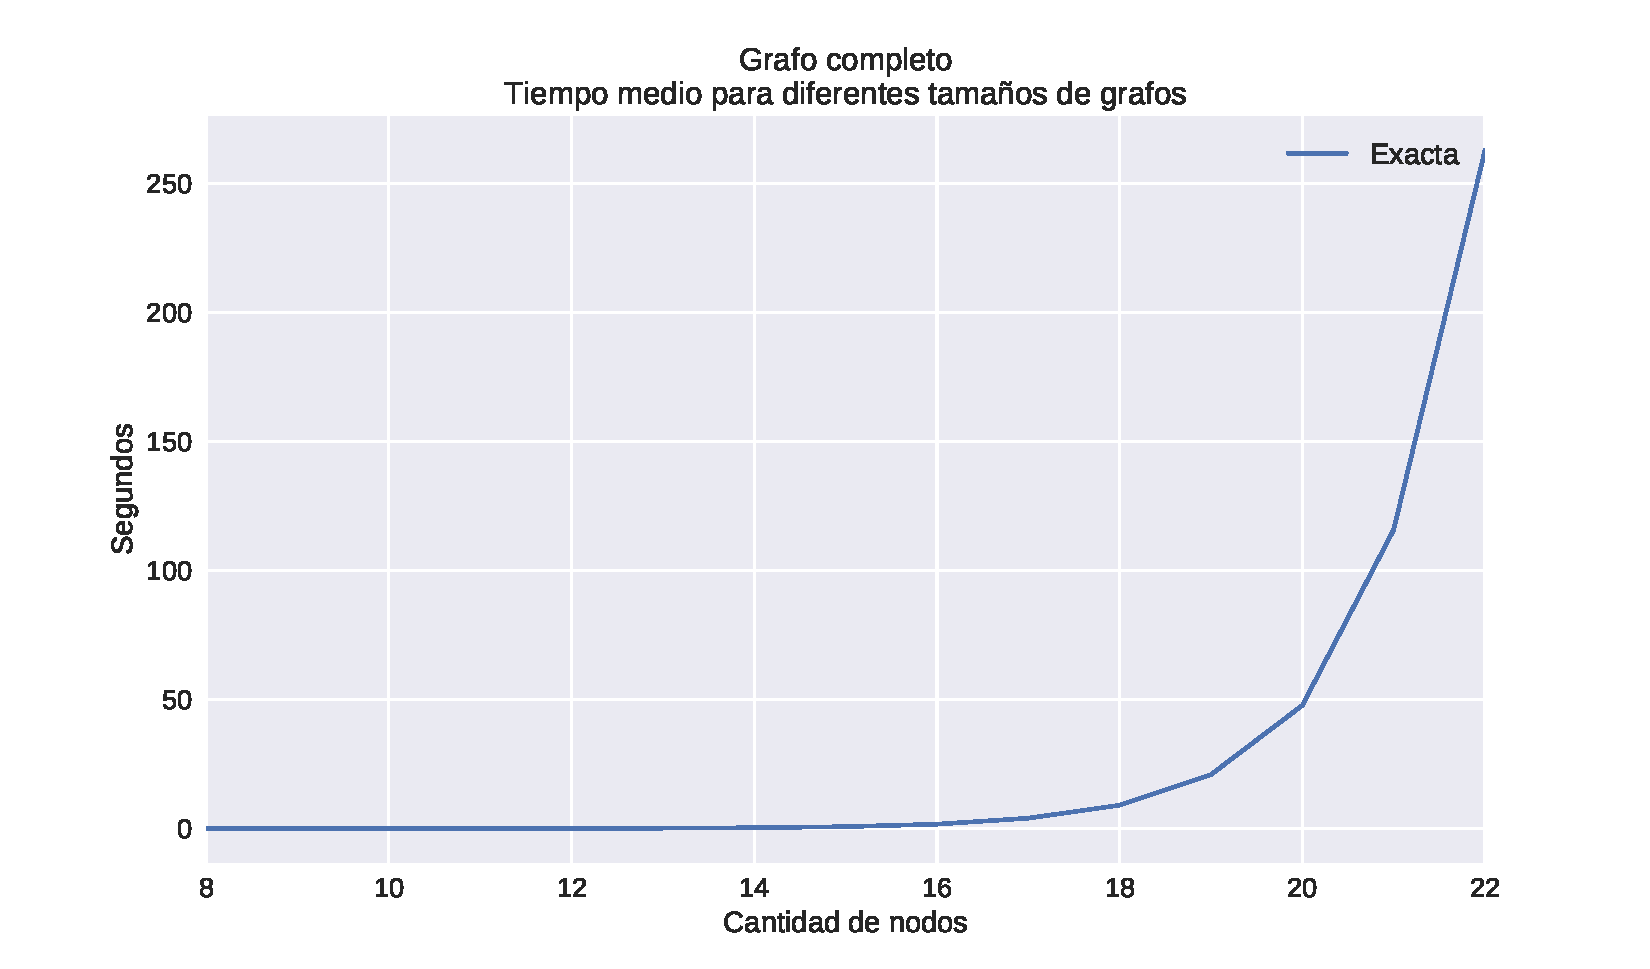
\includegraphics[width=1\textwidth]{informe/imgs/exp_completo_tiempo_exacta.pdf} \\
}

Aprovechemos esta sección para tratar de entender mejor futuras estrategias. Una posible primera idea para de encontrar la clique con máxima frontera, es intentar encontrar la clique máxima. Esta es una \textit{pésima} idea, porque si consideramos un grafo completo de $n$ nodos, la clique máxima es $K_n$ con una frontera de tamaño 0. \\

Vemos en el caso particular de los grafos completos, que la clique que maximiza la frontera tiene tamaño $n/2$. \\

{\centering
    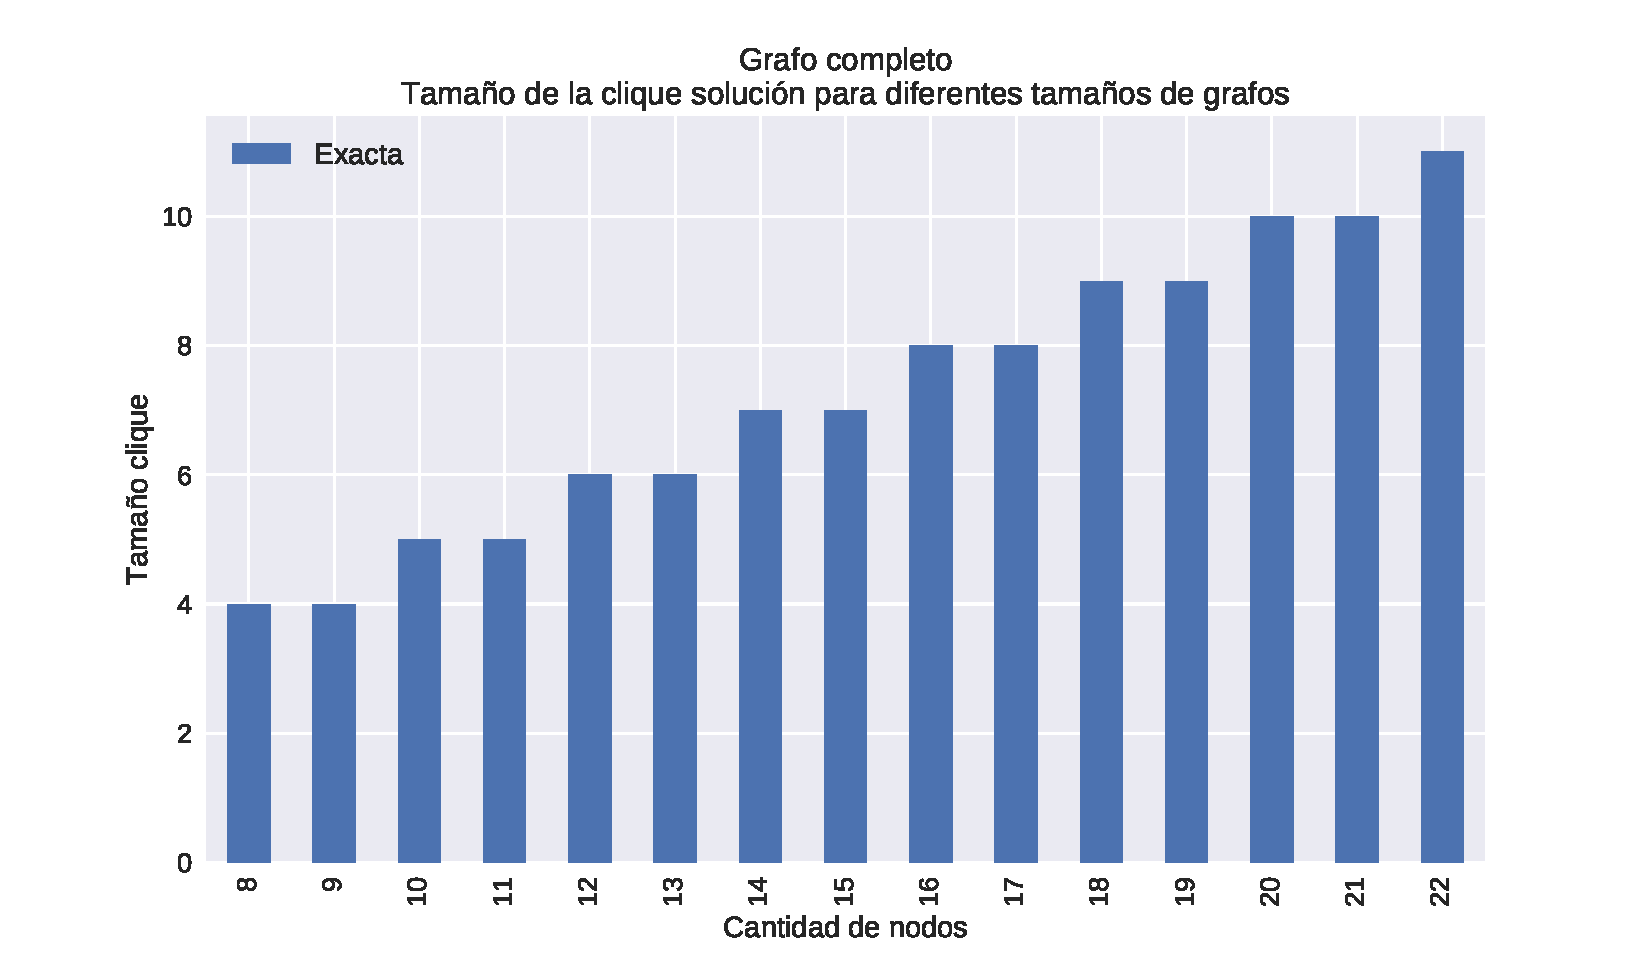
\includegraphics[width=1\textwidth]{informe/imgs/exp_completo_clique_exacta.pdf} \\
}

Como curiosidad, si nuestro grafo es completo no es necesario correr el algoritmo para conocer cuál será la frontera máxima. Basta considerar que la clique que la maximiza tiene $\frac{n}{2}$ nodos, y por cada nodo de la clique hay $\frac{n}{2}$ vecinos exteriores. Por lo tanto, la frontera máxima de un grafo completo es $\frac{n^2}{4}$ \\

Si la clique es demasiado grande, es posible que disminuyamos la cantidad de vecinos que están fuera de la clique. Por lo tanto, la estrategia en las seguientes secciones no será buscar una clique máxima, sino ir construyéndolas pero solo mientras la frontera va aumentando. \\

\todo[inline]{Esto es demasiado lento bla veamos formas aproximadas de resolverlo blabla}

\newpage
% !TEX root = ./informe.tex

\section{Greedy}

\subsection{Explicación}
Teniendo un conjunto solución $S$ que forme una clique, golosamente podemos agregar a $S$ algún nodo que haga aumentar el tamaño de la frontera. \\

Mas detalladamente, el algoritmo funciona de la siguiente manera: \\

Primero considero que todos los nodos son candidatos, y voy a ejecutar el algoritmo siempre que exista algún candidato en la lista. Además mantengo un vector $S$ que representa mi solución actual, inicialmente vacío. Considero que mi frontera máxima $FM$ tiene valor $-1$. \\

Para cada iteracion del ciclo principal, quiero agregar el mejor candidato posible a mi solución. Esto significa iterar por todos mis candidatos y agregar a la solución aquel que maximice la frontera. \\

Recorro mi lista de candidatos y tomo alguno, $c$. Considero $c$ como parte de la solución. Si la solución $S$ no forma una clique, entonces quito $c$ de $S$ , considero que ya no es mas un candidato y vuelvo al comienzo del algortimo. Si $S$ forma una clique, entonces calculo su frontera $f$. \\

Comparo la frontera $f$ con la frontera máxima $FM$. Si $f < FM$, entonces quito a $c$ de $S$, pues no hace que la solucion mejore. Si $f \geq FM$, entonces mantengo a $c$, entonces $c$ es mi mejor candidato, pues la frontera máxima no empeoró. Actualizo $FM$ con el valor de $f$. En ambos casos quito tambíen a $c$ de la lista de candidatos, para no repetirlo dos veces. \\

Una vez encontrado el $c$ que maximice mi solución, lo agrego definitivamente y sigo iterando hasta que ya no pueda considerar mas candidatos. \\

Finalizado el algoritmo, en $S$ va a haber una clique elegida de manera golosa, con la mayor frontera que se puedo encontrar. \\


\subsection{Pseudocódigo}

Referencias de variables globales para el pseudocódigo:
\begin{itemize}
    \item $n$: La cantidad de nodos
    \item $solucion$: Secuencia que contiene la clique solución
    \item $candidatos$: Secuencia con los nodos a considerar
    \item $fronteraMax$: El cardinal de la frontera de la clique solución
\end{itemize}

Las funciones ``EsClique()'' y ``Frontera()'' son las mismas que en el algortimo exacto. Dado que se usan en todos los algoritmos, son omitidas. Tienen complejidad $O(n^3)$ y $O(n^2)$ respectivamente.

\begin{algorithm}[H]
\begin{algorithmic}
\Function{Resolver}{}
    \State LeerInput()                              \Comment $O(n^2)$
    \State $solucion \gets \emptyset$               \Comment $O(1)$
    \State $candidatos \gets \{1, 2, 3, .. , n\} $  \Comment $O(n)$
    \State $fronteraMax \gets -1$                   \Comment $O(1)$
    \State ObtenerSolucion()                        \Comment $O(n^5)$
\EndFunction
\end{algorithmic}
\end{algorithm}



\begin{algorithm}[H]
\begin{algorithmic}
\Function{ObtenerSolucion}{}

    \While{$candidatos \neq \emptyset$}             \Comment $O(n^5)$

        \State $mejorCandidato \gets -1$            \Comment $O(1)$

        \For{$c \in candidatos$}                    \Comment $O(n^4)$
            \State $solucion.push(c)$               \Comment $O(1)$

            \If {$\neg$EsClique($solucion$)}                        \Comment $O(n^3)$
                \State $solucion.erase(c)$                          \Comment $O(n)$
                \State $candidatos.erase(c)$                        \Comment $O(n)$
            \Else
                \State $fronteraActual \gets$ Frontera($solucion$)  \Comment $O(n^2)$
                \If{$fronteraActual \geq fronteraMax$}              \Comment $O(1)$
                    \State $fronteraMax \gets fronteraActual$       \Comment $O(1)$
                    \State $mejorCandidato \gets c$                 \Comment $O(1)$
                \Else
                    \State $candidatos.erase(c)$                    \Comment $O(n)$
                \EndIf

                \State $solucion.erase(c)$                          \Comment $O(n)$
            \EndIf
        \EndFor

        \If{$mejorCandidato \neq -1$}                               \Comment $O(1)$
            \State $solucion.push(mejorCandidato)$                  \Comment $O(1)$
            \State $candidatos.erase(mejorCandidato)$               \Comment $O(n)$

        \EndIf
    \EndWhile

    \State return $solucion$

\EndFunction

\end{algorithmic}
\end{algorithm}

\subsection{Complejidad}

La complejidad principal del algoritmo se encuentra en ``ObtenerSolucion()'', que es $O(n^5)$. Esto es fácil de ver: como nunca se agregan candidatos y siempre se quita al menos uno, el ciclo exterior se ejecuta a lo sumo $O(n)$ veces. El $For$ recorre la lista de candidatos, que son tambien a lo sumo $O(n)$. Dentro del $For$ encontramos solo dos funciones grandes, ``EsClique'' de $O(n^3)$ y ``Frontera'' de $O(n^2)$. El resto son comparaciones, asignaciones y borrados, de $O(n)$. \\

Mas intuitivamente, EsClique ($O(n^3)$) se ejecuta $O(n)$ veces en el For, y a su vez se ejecuta $O(n)$ veces en el While. Por lo tanto, es $O(n^5)$. \\

Si bien $O(n^5)$ puede parecer un polinomio ``grande'', es exponencialmente mejor que el algortimo exacto que tenía $O(2^{n} * n^{3})$. El trade-off es que no siempre se producen soluciones óptimas, como veremos más adelante. \\

\subsection{Optimalidad}

Como podrá verse mas adelante, las soluciones para grafos aleatorios son bastante buenas, pero existe al menos un tipo específico de grafos donde la diferencia entre el exacto y el greedy puede ser \textbf{arbitrariamente grande}. \\

Veamos como podemos construir este tipo de grafos. Vamos a aprovecharnos de que el algoritmo greedy recorre los nodos en orden: 1, 2, 3, 4. \\

{\centering
    
\includegraphics[width=0.57\textwidth]{informe/imgs/greedy_base.png} \\
    \captionof{figure}{Grafo inicial}
}

$ $\newline

Agreguemos 6 vecinos al nodo 1 y agreguemos 4 vecinos a los nodos 2 y 3. El algoritmo goloso toma el primer nodo como solución inicial, es el que tiene mas vecinos. Luego intenta agregar nodos a la solucion de forma tal que formen clique y que tengan mayor frontera. Esto no puede suceder: lo mejor que puede obtener el algoritmo goloso es una clique con frontera de tamaño 7. Sin embargo, podemos ver que la solución óptima está formada por la clique con los nodos 2 y 3, con una frontera de tamaño 9.\\

{\centering
    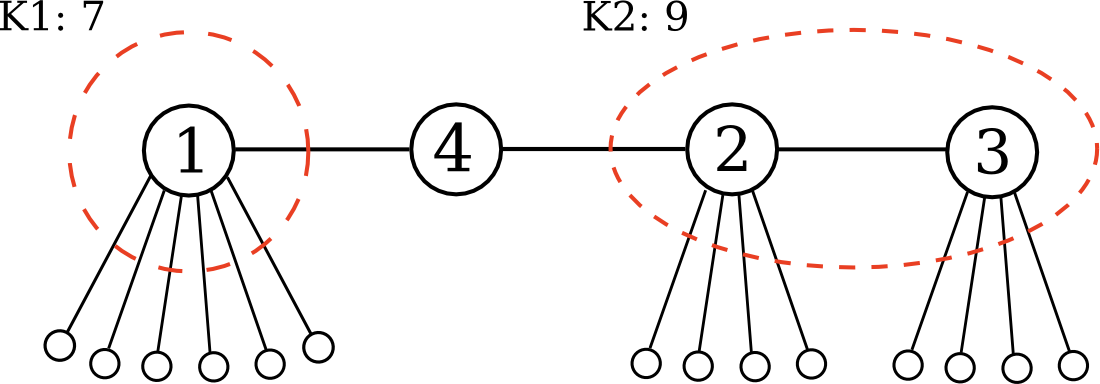
\includegraphics[width=0.57\textwidth]{informe/imgs/greedy_base_nodes_v1.png} \\
}
$ $\newline

Este es un procedimiento que podemos seguir repitiendo. Agregamos un vecino al nodo 1, y un vecino a los nodos 2 y 3. La frontera máxima golosa aumenta en 1, mientras que la frontera máxima aumenta en 2. De esta forma, podemos construir grafos donde la diferencia entre la solución óptima y la solución golosa sea arbitrariamente grande. \\

{\centering
    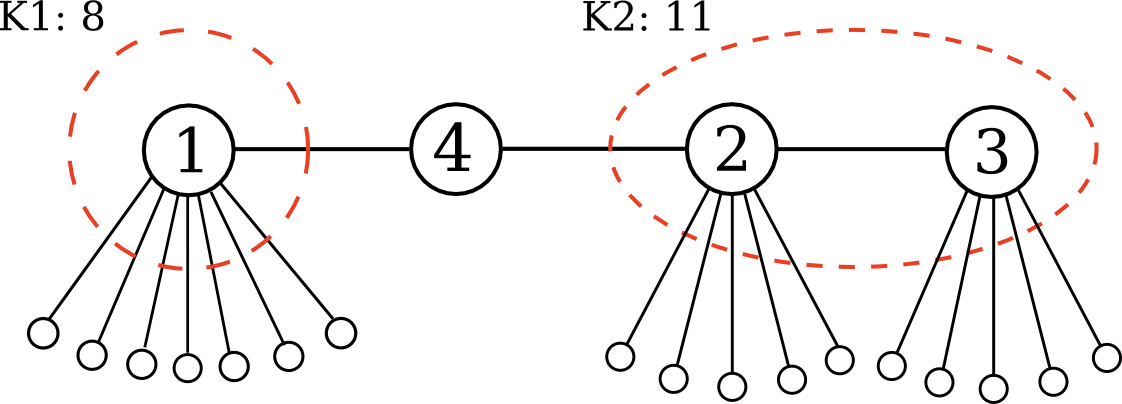
\includegraphics[width=0.57\textwidth]{informe/imgs/greedy_base_nodes_v2.png} \\
}

\subsection{Experimentación}

\todo[inline]{Ver variaciones con entradas malas (item anterior)}


\newpage
% !TEX root = ./informe.tex
\section{Búsqueda Local}

\subsection{Explicación}

Búsqueda local es una estrategia utilizada para mejorar una solución obtenida con una heurística. La idea general es dar una definición de vecindad para toda solución (por ejemplo, si mis soluciones son nodos, los vecinos pueden ser sus adyacentes), y buscar el candidato óptimo dentro de ese conjunto. Este proceso puede repetirse para tender hacia un máximo local. \\

Para este problema particular consideramos que todo clique es solución, y que en su vencindad se encuentran aquellos cliques que pueden obtenerse aplicando una operación de swap (reemplazar un nodo en la clique por uno que no está), una operación de agregado (de un nodo) o una operación de borrado (de un nodo). En cada iteración del algoritmo, revisamos toda la vecindad y nos quedamos con la clique de mayor frontera. La solución final de la búsqueda local es la mejor de las tres posibilidades de nuestra vecindad. \\

\subsection{Pseudocódigo}

Las funciones EsClique() y Frontera() no son incluidas aquí por ser iguales a las incluidas previamente. Las complejidades son $O(n^3)$ y $O(n^2)$ respectivamente. \\

\begin{algorithm}[H]
\begin{algorithmic}
\Function{Resolver}{$solucion$, $iteraciones$}          \Comment $O(iteraciones * n^5)$

    \State $fronteraMaxima \gets$ Frontera($solucion$)                      \Comment $O(n^2)$
    \For{$i \in [1..iteraciones]$ }                                         \Comment $O(iteraciones * n^5)$
        \State $solucionActual \gets$ BusquedaLocal($solucion$)             \Comment $O(n^5)$
        \State $fronteraActual \gets$ Frontera($solucionActual$)            \Comment $O(n^2)$

        \If{$fronteraActual > fronteraMaxima$}                              \Comment $O(1)$
            \State $fronteraMaxima \gets fronteraActual$                    \Comment $O(1)$
            \State $solucion \gets solucionActual$                          \Comment $O(1)$
        \EndIf
    \EndFor
    \State return $solucion$

\EndFunction
\end{algorithmic}
\end{algorithm}


\begin{algorithm}[H]
\begin{algorithmic}
\Function{BusquedaLocal}{$solucionInicial$}             \Comment $O(n^5)$
    \State $complementoInicial \gets$ Complemento($solucionInicial$) \Comment $O(n)$\\

    \State $solucionSwap \gets$ MaximoPorSwap($solucionInicial$, $complementoInicial$)  \Comment $O(n^5)$
    \State $fronteraSwap \gets$ Frontera($solucionSwap$)                                \Comment $O(n^2)$ \\

    \State $solucionAdd \gets$ MaximoPorAdd($solucionInicial$, $complementoInicial$)    \Comment $O(n^4)$
    \State $fronteraAdd \gets$ Frontera($solucionAdd$)                                  \Comment $O(n^2)$\\

    \State $solucionSub \gets$ MaximoPorSub($solucionInicial$)      \Comment $O(n^4)$
    \State $fronteraSub \gets$ Frontera($solucionSub$)              \Comment $O(n^2)$\\

    \State $solucionSuprema \gets solucionSwap$ \Comment $O(1)$
    \State $fronteraSuprema \gets fronteraSwap$ \Comment $O(1)$\\

    \If{$fronteraAdd > fronteraSuprema$}                \Comment $O(1)$
        \State $fronteraSuprema \gets$ $fronteraAdd$    \Comment $O(1)$
        \State $solucionSuprema \gets$ $solucionAdd$    \Comment $O(1)$\\
    \EndIf

    \If{$fronteraSub > fronteraSuprema$}                \Comment $O(1)$
        \State $fronteraSuprema \gets$ $fronteraSub$    \Comment $O(1)$
        \State $solucionSuprema \gets$ $solucionSub$    \Comment $O(1)$\\
    \EndIf

    \State return $solucionSuprema$                     \Comment $O(1)$
\EndFunction

\end{algorithmic}
\end{algorithm}

Al swappear no nos quedamos con el primer swappeo que se pueda, sino que vemos las $n^2$ combinaciones de swaps para elegir la mejor (siempre que el swap mantenga una clique solución).

\begin{algorithm}[H]
\begin{algorithmic}
\Function{MaximoPorSwap}{$solucionInicial$, $complementoInicial$}   \Comment $O(n^5)$

    \State $candidatos \gets solucionInicial$
    \State $maxFrontera \gets$ Frontera($solucionInicial$)  \Comment $O(n^2)$
    \State $max\_i \gets -1$                                \Comment $O(1)$
    \State $max\_j \gets -1$                                \Comment $O(1)$\\

    \For{$i \in [0..|solucionInicial|)$}                    \Comment $O(n^5)$ Ver sección Complejidad
        \For{$j \in [0..|complementoInicial|)$}

            \State $candidato$[$i$] $\gets complementoInicial$[$j$] \Comment Hacemos swap $O(1)$

            \If{EsClique($candidatos$)}                                         \Comment $O(n^3)$
                \State $fronteraCandidato \gets$ Frontera($candidato$)          \Comment $O(n^2)$
                \If{$fronteraCandidato > maxFrontera$}                          \Comment $O(1)$
                    \State $max\_i \gets i$                                     \Comment $O(1)$
                    \State $max\_j \gets j$                                     \Comment $O(1)$
                    \State $maxFrontera \gets fronteraCandidato$                \Comment $O(1)$
                \EndIf
            \EndIf

            \State $candidato$[$i$] $\gets solucionInicial$[$j$] \Comment Restauro swap $O(1)$
        \EndFor
    \EndFor

    \If{$max\_i \neq -1$}                           \Comment $O(1)$
        \State $candidato$[$max\_i$] $\gets$ $complementoInicial$[$max\_j$] \Comment Swapeo definitivamente $O(1)$
    \EndIf

    \State return $candidatos$                      \Comment $O(1)$

\EndFunction
\end{algorithmic}
\end{algorithm}

En ``MaximoPorSub'' calculamos la frontera al sacar un único nodo (lo hacemos para todos los nodos) y vemos si la frontera aumenta. Puede pasar que al disminuir el tamaño de una clique queden muchas aristas ``libres'' que hagan que la frontera aumente. Probamos con todos y nos quedamos con la respuesta que mejoró la frontera, si es que hubo alguna.

\begin{algorithm}[H]
\begin{algorithmic}
\Function{MaximoPorSub}{$solucionInicial$}                      \Comment $O(n^4)$
    \State $candidatos \gets solucionInicial$
    \State $maxFrontera \gets$ Frontera($solucionInicial$)      \Comment $O(n^2)$
    \State $max\_c \gets -1$  \\                                \Comment $O(1)$

    \For{$c \in candidatos$}                                                \Comment $O(n^4)$
        \If{EsClique($candidatos - \{c\}$)}                                 \Comment $O(n^3)$
            \State $fronteraCandidato \gets$ Frontera($candidatos - \{c\}$) \Comment $O(n^2)$
            \If{$fronteraCandidato > maxFrontera$}                          \Comment $O(1)$
                \State $max\_c \gets c$                                     \Comment $O(1)$
                \State $maxFrontera \gets fronteraCandidato$                \Comment $O(1)$ \\
            \EndIf
        \EndIf
    \EndFor

    \If{$max\_c \neq -1$}                                           \Comment $O(1)$
        \State $candidatos \gets (candidatos - \{max\_c\})$         \Comment $O(1)$
    \EndIf

    \State return $candidatos$

\EndFunction
\end{algorithmic}
\end{algorithm}

En ``MaximoPorAdd'' probamos agregar de a un nodo, viendo que forme clique y calculando la nueva frontera. Si la frontera aumenta, nos guardamos la nueva solución.

\begin{algorithm}[H]
\begin{algorithmic}
\Function{MaximoPorAdd}{$solucionInicial$, $complementoInicial$}        \Comment $O(n^4)$

    \State $maxFrontera \gets$ Frontera($solucionInicial$)              \Comment $O(n^2)$
    \State $max\_c \gets -1$                                            \Comment $O(1)$
    \State $candidatos \gets solucionInicial$                           \Comment $O(1)$\\

    \For{$c \in complementoInicial$}                                            \Comment $O(n^4)$
        \If{EsClique($candidatos + \{c\}$)}                                     \Comment $O(n^3)$
            \State $fronteraCandidato \gets$ Frontera($candidatos + \{c\}$)     \Comment $O(n^2)$
            \If{$fronteraCandidato > maxFrontera$}                              \Comment $O(1)$
                \State $max\_c \gets c$                                         \Comment $O(1)$
                \State $maxFrontera \gets fronteraCandidato$                    \Comment $O(1)$\\
            \EndIf
        \EndIf
    \EndFor

    \If{$max\_c \neq -1$}                                           \Comment $O(1)$
        \State $candidatos \gets (candidatos + \{max\_c\})$         \Comment $O(1)$
    \EndIf

    \State return $candidatos$                      \Comment $O(1)$

\EndFunction
\end{algorithmic}
\end{algorithm}

Para calcular el complemento, armamos un vector de booleanos que dicen si un nodo pertenece o no a la solución input. Luego recorremos el vector y armamos un nuevo vector con aquellos nodos que no estaban en la solución original.

\begin{algorithm}[H]
\begin{algorithmic}
\Function{Complemento}{$solucionInicial$}
    \State $pertenece[i] =$ True $\iff i \in solucionInicial$   \Comment $O(n)$
    \State $complemento \gets \{\}$                             \Comment $O(1)$

    \For{$i \in [0..n)$}                                        \Comment $O(n)$
        \If{$pertenece$[$i$]$ = $True}                          \Comment $O(1)$
            \State $complemento$.PushBack($i$)                  \Comment $O(1)$  amortizado
        \EndIf
    \EndFor

    \State return $complemento$                                 \Comment $O(1)$

\EndFunction
\end{algorithmic}
\end{algorithm}


\subsection{Complejidad}

Las complejidades de cada linea fueron marcadas en el pseudocódigo, por lo que calcular la complejidad total es bastante sencillo.

\begin{itemize}
    \item MaximoPorAdd: $O(n^4)$. Son $O(n)$ iteraciones de algo $O(n^3)$.
    \item MaximoPorSub: $O(n^4)$. Son $O(n)$ iteraciones de algo $O(n^3)$.
    \item MaximoPorSwap: $O(n^5)$. El primer For recorre un vector $v$ y el For anidado recorre su complemento. Si consideramos que $|v| = \frac{n}{2}$, entonces el tamaño del complemento también es $\frac{n}{2}$, por lo que en total se recorren $O(n^2)$ elementos. Son $O(n^2)$ iteraciones de algo $O(n^3)$.
    \item BusquedaLocal: $O(n^5)$. Esto es por la complejidad de MaximoPorSwap que es la mayor, todo el resto es $O(n^4)$ o menor.
    \item Resolver: $O(\#iteraciones * n^5)$. Son $\#iteraciones$ veces de BusquedaLocal.
\end{itemize}

Por lo tanto, mejorar una solución inicial con este algoritmo de búsqueda local cuesta $O(\#iteraciones * n^5)$.

\subsection{Optimalidad}

Algo que notamos al probar este método es que el algoritmo goloso presentado en la sección anterior ya llega a un máximo local, por lo que es redundante aplicarle una búsqueda local para mejorarla. ¿Por qué ocurre esto? Porque si hubiera un nodo al que swappear con alguna de afuera para conseguir una mejor frontera, como este algoritmo siempre se queda con el mejor nodo fuera de la clique, entonces el nodo de afuera ya tendría que estar dentro de la clique. Tampoco podemos agregar nodos, pues si pudiesemos tomar más, el algoritmo goloso ya lo hubiera hecho.  \\

% Lo siento, no hay tiempo
% \todo{Mmm... No se me ocurre que pasa con Sub}

Sin embargo, aún así podemos encontrarle un uso. En la sección de Optimalidad del algoritmo goloso notamos que la diferencia entre la solución proporcionada por el algoritmo y la solución real puede ser arbitrariamente grande, con lo cuál pueden haber casos muy malos para nuestro algoritmo. Una forma de paliar este problema es que el algoritmo tome como entrada un nodo inicial, y que a partir de ahí construya una solución golosa. Llamaremos a esta variante $golosoB$, y al original $golosoA$. Por cuestiones de tiempo y del alcance de este informe no detallaremos la implementación de $golosoB$, pero es el algoritmo que motivará este apartado. Sin embargo, no es más que lo que acabamos de decir, es sencillamente fijar un nodo incial antes de aplicar el algoritmo. \\

¿Por qué sirve nuestro algoritmo de búsqueda local para $golosoB$? Esto ocurre porque el primer nodo no fue elegido golosamente, es un nodo arbitrario que fijamos en nuestra solución. Como consecuencia, una vez que la solución golosa queda construida, eliminar o swappear el primer nodo podría llegar producir un aumento en la frontera (agregar no, pues el algoritmo goloso siempre llega a un máximo local respecto a esta operación). Si esto llegase a ocurrir, aparecerían nuevos nodos candidatos a entrar en nuestra solución que no podiamos tomar antes porque no estaban conectados con el primer nodo. De esta forma, podemos continuar moviéndonos por las soluciones para llegar a algún máximo local incluso mejor que el nos devolvió $golosoA$. \\

Tomemos el mismo ejemplo que complicaba a $golosoA$ utilizando $golosoB$ utilizado en \textit{búsquedaLocal}. \\

{\centering
    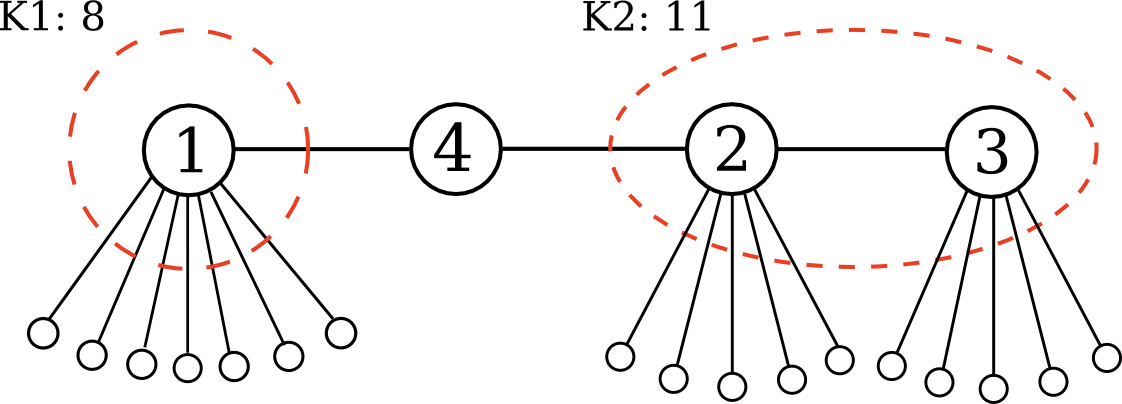
\includegraphics[width=0.57\textwidth]{informe/imgs/greedy_base_nodes_v2.png} \\
}
$ $\newline

Si a $golosoB$ le pasamos como entrada un nodo perteneciente al arbol $1$, o el nodo $4$; es imposible mejorar la solución de $golosoA$. Es el riesgo que tenemos al dejar libre el nodo inicial. Es importante notar que la solución \textbf{no} es peor, sino que simplemente no se mejora. \textit{-Desarrollaremos un poco más en unos párrafos-.} Sin embargo, si elegimos un nodo cualquiera del arbol $2$ o $3$, la situación es distinta. \\

El caso fácil es si elegimos los nodos $2$ o $3$, en donde $golosoB$ se queda con la solución $[2,3]$, ya que ni las hojas ni el cuatro generan una clique con mayor frontera que ese par de nodos, mejorando la anterior solución. \\

Más complicado es lo que ocurre al tomar una hoja de los arboles $2$ y $3$ como inicial. Asumamos que tomamos una hoja del $2$ (tomar una hoja del $3$ es análogo). La hoja sólo está conectada con el $2$, por lo que el $2$ se incluye en la solución. Una vez realizado esto, como nadie más está conectado con la hoja, \textit{golosoB} devuelve $[hoja,2]$. Es en este caso en donde \textit{búsquedaLocal} ayuda, pues a partir de $[hoja,2]$ busca los cliques que se pueden obtener haciendo swaps, con lo cual considera como candidato al clique producto de swappear la $hoja$ con el $2$, que es la clique $[2,3]$. Al ser la solución óptima, el algoritmo la toma en la primera iteración, y corta en la segunda. Termina devolviendo lo que queriamos: $[2,3]$. \\

{\centering
    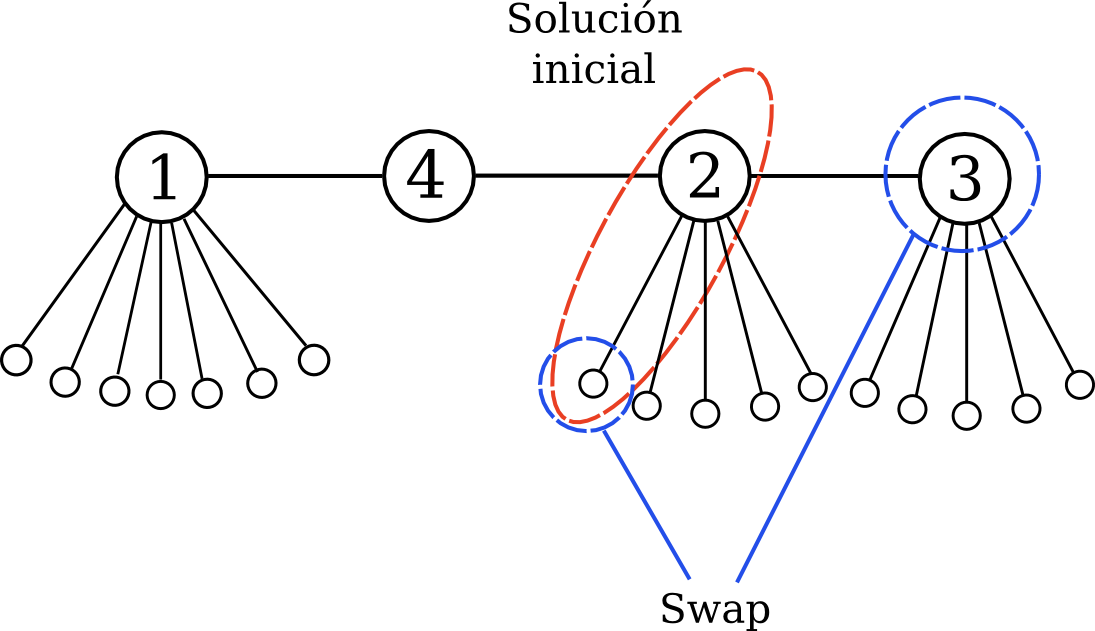
\includegraphics[width=0.57\textwidth]{informe/imgs/local_base_nodes_v2.png} \\
}
$ $\newline

{\centering
    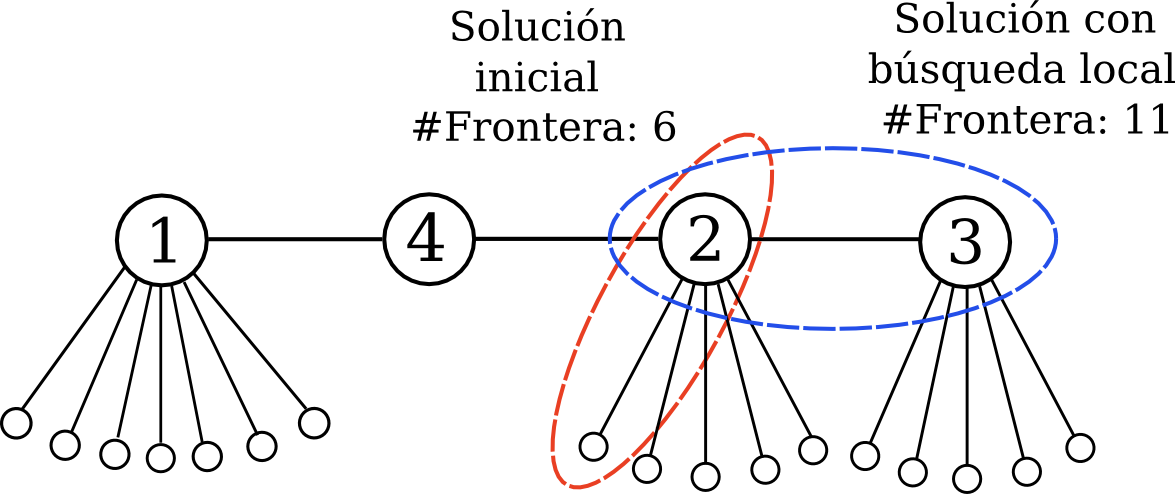
\includegraphics[width=0.57\textwidth]{informe/imgs/local_base_nodes_v3.png} \\
}
$ $\newline

Retomando lo mencionado hace unos párrafos, ¿que sucede si se elije un nodo del árbol $1$? Claramente $golosoB$ se vuelve tan malo como $golosoA$, pero \textbf{existe una solución muy sencilla}: podríamos elegir al azar el nodo inicial y correr el algoritmo muchas veces, para quedarnos con la mejor. Con sufieciente cantidad de elecciones, es esperable que se elimine el problema de empezar con nodos que no pueden seguir mejorándose. Exploraremos esta idea en la última sección del informe: $GRASP$.

\subsection{Experimentación}

Como contamos antes, el algoritmo goloso que utilizamos en búsqueda local depende de un nodo inicial. Creemos que la muestra mas representativa para \textit{grafos malos} se obtiene partiendo de un nodo al azar. Lo que hicimos para conseguir los datos es para cada tamaño de $n$, correr 50 veces el experimento y quedarnos con la media de los datos, lo que explica las fuertes variaciones de la curva. Con esto queda claro que esta técnica en promedio proporciona mejores resultados, es muy dependiente del nodo inicial. Intentaremos solucionar este problema en el siguiente apartado. \\

Es claro que al aplicar búsqueda local se agregan muchas operaciones extra que antes no existían, por lo que es esperable que el tiempo de ejecución aumente. Una posible pregunta es ¿Cómo influye en esto la cantidad de iteraciones? ¿Aumenta el tiempo al punto de hacerlo inutilizable? \textbf{Los siguientes gráficos fueron realizados tomando el grafo malo que presentamos anteriormente}.

{\centering
    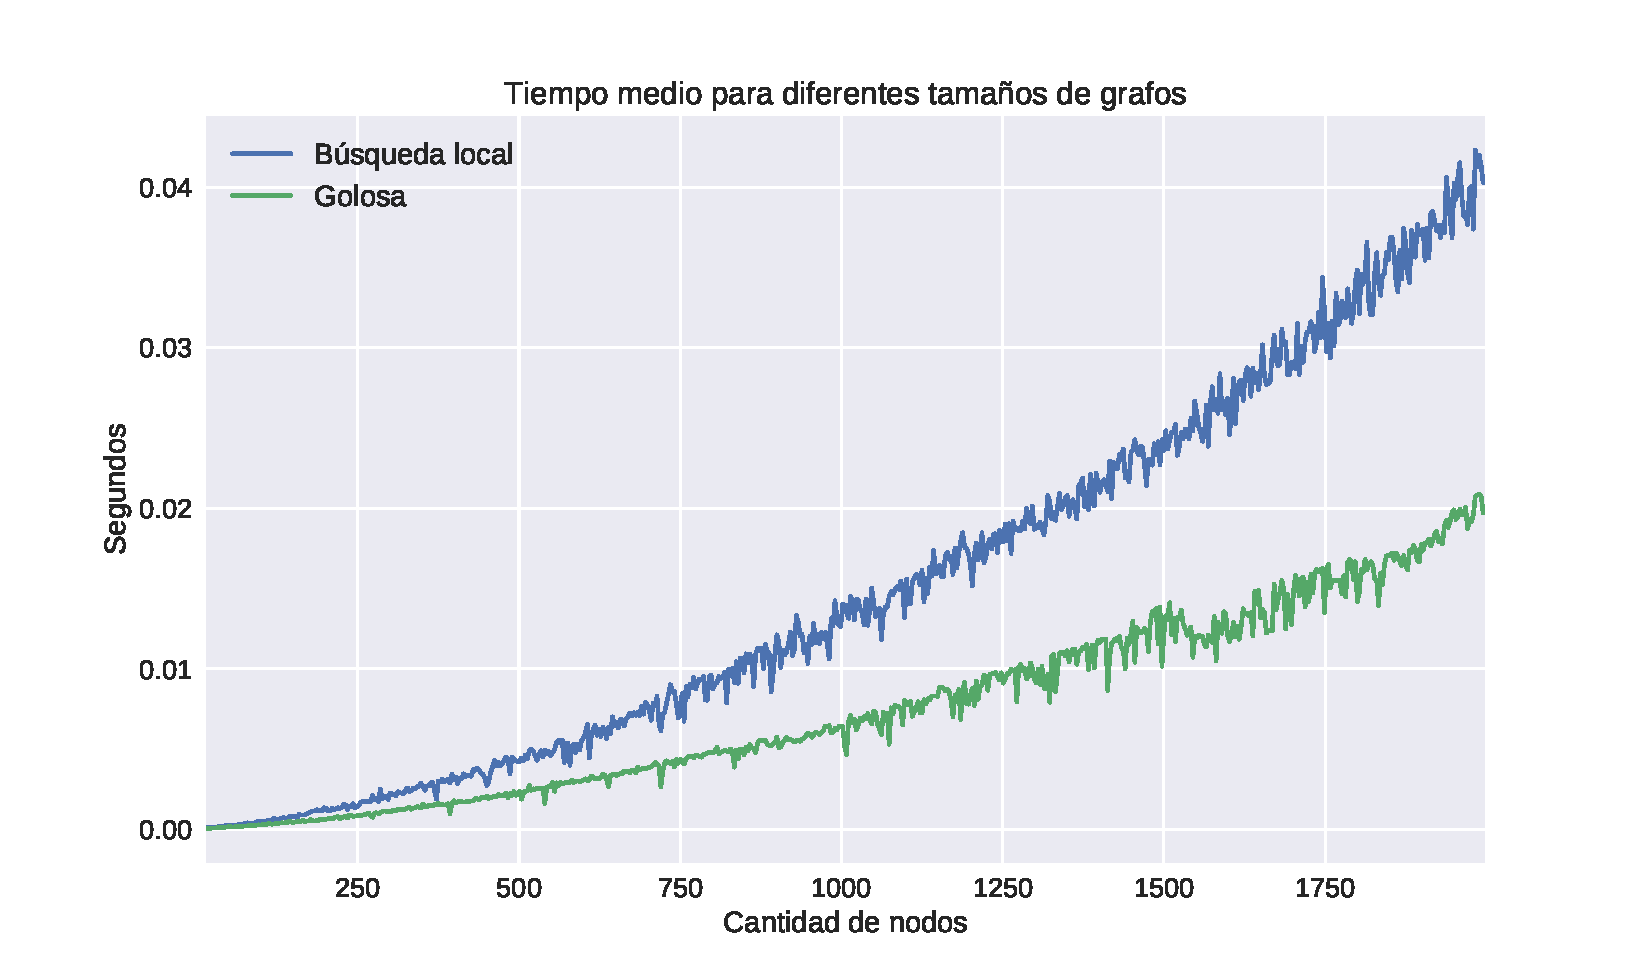
\includegraphics[width=1\textwidth]{informe/imgs/exp_malo_tiempo_greedy_local.pdf}
    \captionof{figure}{$\uparrow$ 10 iteraciones.}
}
{\centering
    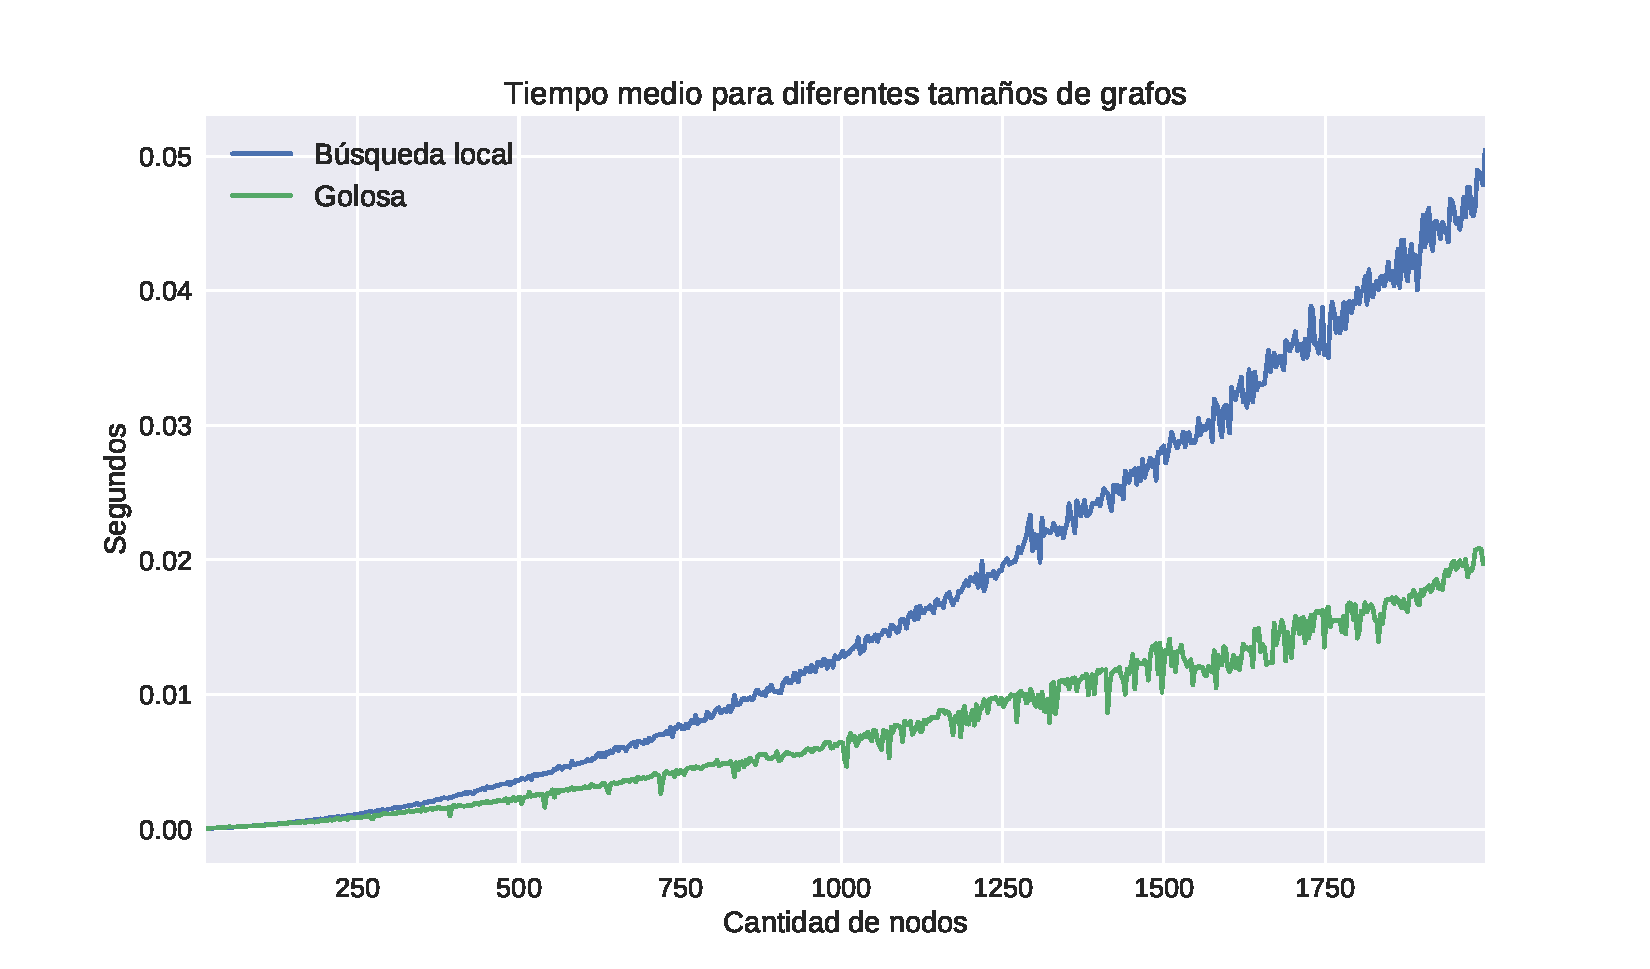
\includegraphics[width=1\textwidth]{informe/imgs/exp_malo_tiempo_greedy_local_2000.pdf}
    \captionof{figure}{$\uparrow$ 2000 iteraciones.}
}
$ $\newline

El primer gráfico fue realizado con $10$ iteraciones, mientras que el segundo fue obtenido con $2000$ iteraciones. Si bien el tiempo en el de $2000$ es mayor, lo es solo por una \textit{pequeña} diferencia. Lo que sucede es que nuestro algoritmo deja de ejecutarse cuando se estanca en un extremo local, pues una vez dentro ya no tiene forma de escapar. \\

La siguiente pregunta que surge es, ¿mejoramos la solución del caso malo? Considerando una búsqueda local de 2000 iteraciones, veamos como es la solución promedio. \\

{\centering
    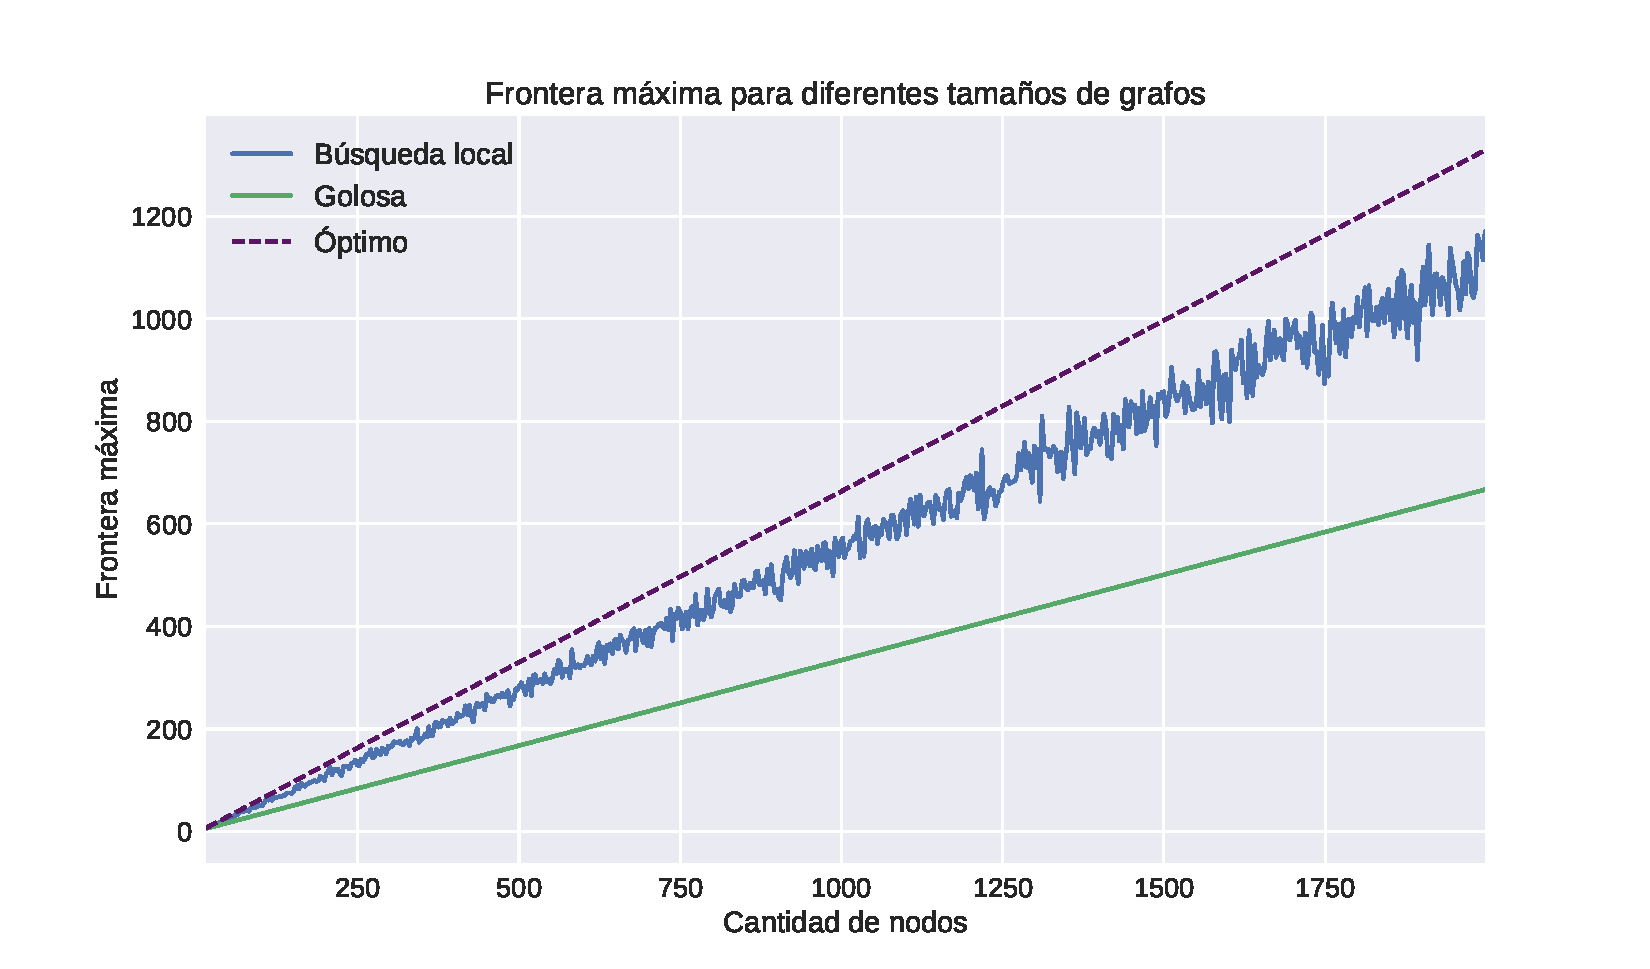
\includegraphics[width=1\textwidth]{informe/imgs/exp_malo_frontera_greedy_local_2000_optimo.pdf}
}

% Mas de lo mismo
% {\centering
%     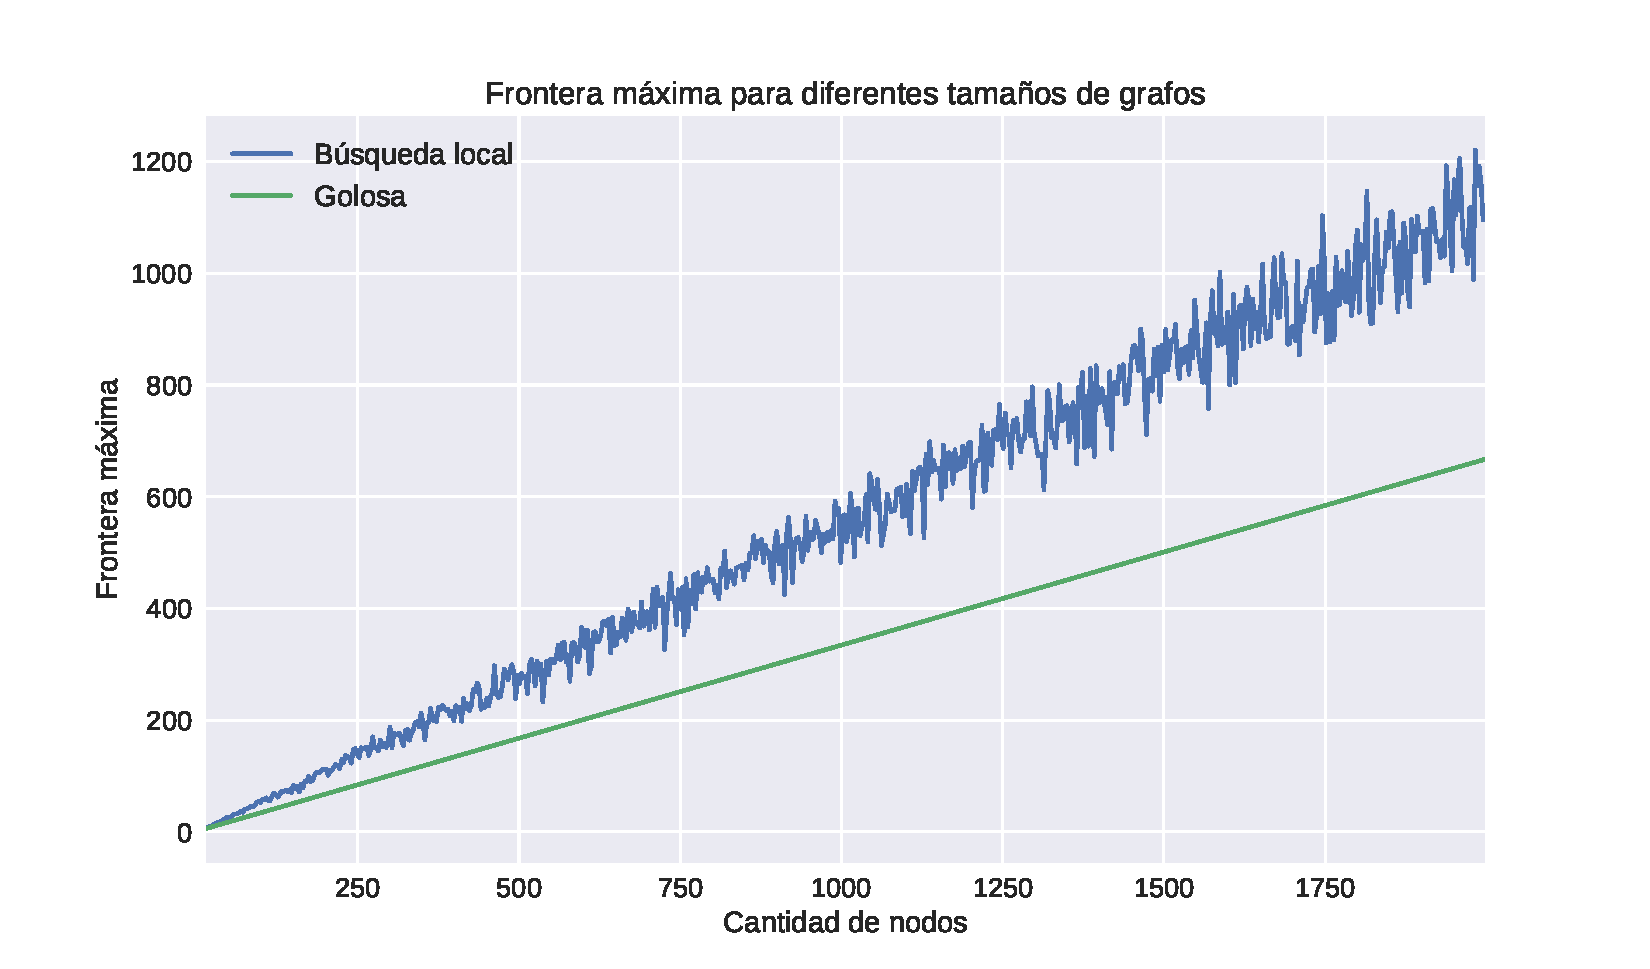
\includegraphics[width=1\textwidth]{informe/imgs/exp_malo_frontera_greedy_local.pdf} \\
% }
% $ $\newline
Recordemos que por construcción, en la sección anterior pudimos calcular analiticamente cuál era la solución óptima para cada $n$ de nuestros \textit{grafos malos}. Recordemos también que lo que graficamos es \textbf{el promedio} de las soluciones, es decir, \textit{en realidad hay soluciones que alcanzan al óptimo}, pero muchas otras que no. Con una cantidad suficiente de repeticiones vemos que el promedio se encuentra aproximadamente en el centro: por ese motivo decimos que en promedio no consigue la solución óptima. \\

En general con búsqueda local se logró una mejora con respecto a la solución golosa, pero no lo suficiente. Sigue siendo un método que está condenado a caer en extremos locales, y una vez dentro no puede escapar. La motivación de la siguiente sección será intentar resolver esta falencia.


\newpage
% !TEX root = ./informe.tex
\section{Grasp}

\subsection{Explicación}
GRASP es sigla de Procedimientos Golosos Aleatorios Adaptativos de Búsqueda (Greedy Randomized Adaptive Search Procedures). Es una metaheurística que se basa en utilizar métodos golosos constructivos y de búsqueda local para resolver problemas computacionalmente difíciles, utilizando el azar para evitar estancarse en un único máximo local. Cada iteración de un algoritmo GRASP construye golosamente una solución desde cero, admitiendo cierto grado de aleatoriedad al añadir elementos, para después mejorarla con un método de búsqueda local. Realizamos varias iteraciones deteniéndonos bajo algún criterio de corte, ya sea por que conseguimos una solución lo suficientemente buena o porque nos pasamos de una cantidad de iteraciones predeterminada. La mejor solución conseguida entre todas las iteraciones es el resultado final del algoritmo. \cite{paper_grasp} \\

El algoritmo goloso constructivo que vamos a utilizar va a ir un poco más allá del algoritmo \textit{golosoB} del que hablamos en la sección anterior. En vez de maximizar de forma directa nuestra función greedy (cardinalidad de la frontera) sobre los nodos no agregados, construiremos un conjunto de candidatos llamado RCL (Restricted Candidate List). La misma contendrá los candidatos que cumplan con un cierto nivel de optimalidad, del que será elegido un nodo al azar para ser agregado a la solución final. \\

El criterio con el cuál se tomarán candidatos al RCL estará dictaminado por un parámetro $alpha$, que indicará qué porcentaje del rango de valores posibles que pueden tomar los candidatos se admiten en la RCL. Formalmente, un nodo $c$ que resulta en una frontera $f_c$ al ser agregado a la solución parcial, pertenece al RCL solo si $f_c \geq f_{max} + \alpha * (f_{min} - f_{max})$, con $max$ nodo localmente óptimo, y $min$ nodo localmente peor. A grandes rasgos, un $alpha$ grande implica darle más peso al azar, y uno más chico, a la porción golosa del algoritmo. (Notemos que para que esto tenga sentido, $\alpha \in \mathbb{R}$ y $0 \leq \alpha \leq 1$). Una vez que el RCL está formado, se elije un nodo al azar, y se comienza el proceso de nuevo, hasta no poder continuar. \\

Obtenida una solución inicial, como nuestro método no es (en general) completamente goloso, podemos utilizar un algoritmo de búsqueda local para movernos hacia un máximo local, mejorando nuestra solución y completando una iteración de GRASP. El algoritmo que usamos para este propósito es el mismo de la sección anterior.

\subsection{Pseudocódigo}

Las funciones local.resolver(), EsClique() y Frontera() no son incluidas aquí por ser iguales a las incluidas previamente. Las complejidades son $O(n^5)$, $O(n^3)$ y $O(n^2)$ respectivamente.

Referencias de variables globales para el pseudocódigo:
\begin{itemize}
    \item $n$: La cantidad de nodos
    \item $solucion$: Secuencia que contiene la clique solución
\end{itemize}

\begin{algorithm}[H]
\begin{algorithmic}
\Function{Resolver}{$\alpha$, $repsGrasp$, $repsLocal$}
    \State $fronteraMax \gets 0$                    \Comment $O(1)$
    \State $fronteraNueva \gets 0$                  \Comment $O(1)$
    %\State $reps \gets 0$                           \Comment $O(1)$
    \For{$reps \in$ [$1..repsGrasp$]}                           \Comment $O(repsGrasp * repsLocal * n^5)$
    % \While{$reps < repsGrasp$}  \Comment $What Goes Here$
        \State $actual \gets $GreedyRandom($\alpha$)              \Comment $O(n^5)$
        \State $nueva \gets$ local.resolver($actual, repsLocal$)  \Comment $O(repsLocal * n^5)$
        \State $fronteraNueva \gets$ Frontera($nueva$)            \Comment $O(n^2)$
        \If {$fronteraNueva > fronteraMax$}                     \Comment $O(1)$
            \State $solucion \gets nueva$                       \Comment $O(1)$
            \State $fronteraMax \gets fronteraNueva$            \Comment $O(1)$
        %     \State $reps \gets 0$   \Comment $O(1)$
        % \Else
        %     \State $reps \gets reps + 1$   \Comment $O(1)$
        \EndIf
    % \EndWhile
    \EndFor
    \State return $solucion$
\EndFunction
\end{algorithmic}
\end{algorithm}
Para calcular el $RCL$ hacemos un primer pasaje para calcular el máximo y el mínimo de los nodos candidatos a agregarse al clique parcial. En una segunda pasada es cuando vamos agregando los nodos a medida que encontramos aquellos que cumplen con la fórmula planteada en la Explicación.

\begin{algorithm}[H]
\begin{algorithmic}
\Function{GreedyRandom}{$\alpha$}
    \State $fronteraMax \gets -1$                       \Comment $O(1)$

    \State $candidatosInicial \gets \{1..n\}$         \Comment $O(n)$

    \State $solucion \gets \emptyset$                   \Comment $O(1)$

    \State $puedoConstruirClique \gets$ True            \Comment $O(1)$ \\

    \While {$puedoConstruirClique \land |candidatosInicial| > 0$}   \Comment $O(n^5)$
        \State $puedoConstruirClique \gets$ False                        \Comment $O(1)$

        \State $candidatos \gets \emptyset$   \Comment $O(1)$
        \State $RCL \gets \emptyset$          \Comment $O(1)$ \\

        \For {$c \in candidatosInicial$}                                \Comment $O(n^4)$
            \If {EsClique($solucion + \{c\}$)}                          \Comment $O(n^3)$
                \State $front \gets$ Frontera($solucion$)               \Comment $O(n^2)$
                \State $candidatos \gets candidatos + \{(front, c)\}$   \Comment $O(1)$
                \State $puedoConstruirClique \gets$ True                \Comment $O(1)$ \\
            \EndIf
        \EndFor
        \State $fronteraMinTmp \gets \infty$   \Comment $O(1)$
        \State $fronteraMaxTmp \gets -1$   \Comment $O(1)$
        \For {$cand \in candidatos$}   \Comment $O(n)$
            \State $fronteraMinTmp \gets min(fronteraMinTmp, cand.first)$   \Comment $O(1)$
            \State $fronteraMaxTmp \gets max(fronteraMaxTmp, cand.first)$   \Comment $O(1)$ \\
        \EndFor

        \For {$cand \in candidatos$}   \Comment $O(n)$
            \If {$cand.first \geq fronteraMaxTmp + \alpha*(fronteraMinTmp - fronteraMaxTmp)$}   \Comment $O(1)$
                \State $RCL \gets RCL + \{cand.second\}$   \Comment $O(1)$ \\
            \EndIf
        \EndFor

        \If {$puedoConstruirClique$}   \Comment $O(1)$
            \State $randomIndex \gets random(\{1 .. |RCL|\})  $   \Comment $O(1)$
            \State $solucion \gets solucion + \{RCL[randomIndex]\}$   \Comment $O(1)$

            \State $candidatosInicial \gets candidatosInicial - \{RCL[randomIndex]\}$   \Comment $O(1)$ \\
        \EndIf
    \EndWhile
    \State $fronteraMax \gets$ Frontera($solucion$)   \Comment $O(1)$
    \State return $solucion$
\EndFunction
\end{algorithmic}
\end{algorithm}


\subsection{Complejidad}

Analicemos en primer lugar la complejidad de ``GreedyRandom'':
\begin{itemize}
    \item Iteraciones del while son $O(n)$: Se corta cuando $candidatosInicial.size = 0$, y en cada iteración a $candidatosInicial$ se le resta $RCL$, que nunca está vacío pues siempre el nodo golosamente óptimo pertenece, por lo cual la cantidad de iteraciones es $O(n)$.
    \item Calcular fronteras de candidatos es $O(n^4)$: Recorremos la lista de candidatos ($O(n)$), y para cada uno preguntamos si es clique en $O(n^3)$ y si lo es, su frontera en $O(n^2)$.
    \item Calcular fronteras máximas y mínimas es $O(n)$: Calculadas todas las fronteras de los candidatos, solo hay que recorrer esa secuencia y quedarme con el máximo y el mínimo
    \item Construir el RCL es $O(n)$: Consta de recorrer los candidatos y verificar para cada uno si se cumple una fórmula calculable en $O(1)$
\end{itemize}

Entonces, su complejidad es:

$$ O(n) * (O(n^4) + O(n^3) + O(n)) = O(n^5)$$

Con esta información en mano, el grueso de la complejidad de GRASP proviene simplemente de aplicar ``GreedyRandom'' y luego ``BusquedaLocal'' que son ambas $O(n^5)$ (aunque busqueda local también depende de una cantidad de iteraciones), un número $repsGrasp$ de veces. Por ende, la complejidad final del algoritmo es O($repsGrasp * repsLocal * n^5$).

% Creo que no hay nada que decir para merecer una seccion "optimalidad". Si alguien tiene algo sea libre, pero en gral trato todo al analizar los experimentos.
% \subsection{Optimalidad}

\subsection{Experimentación}

% {\centering
%     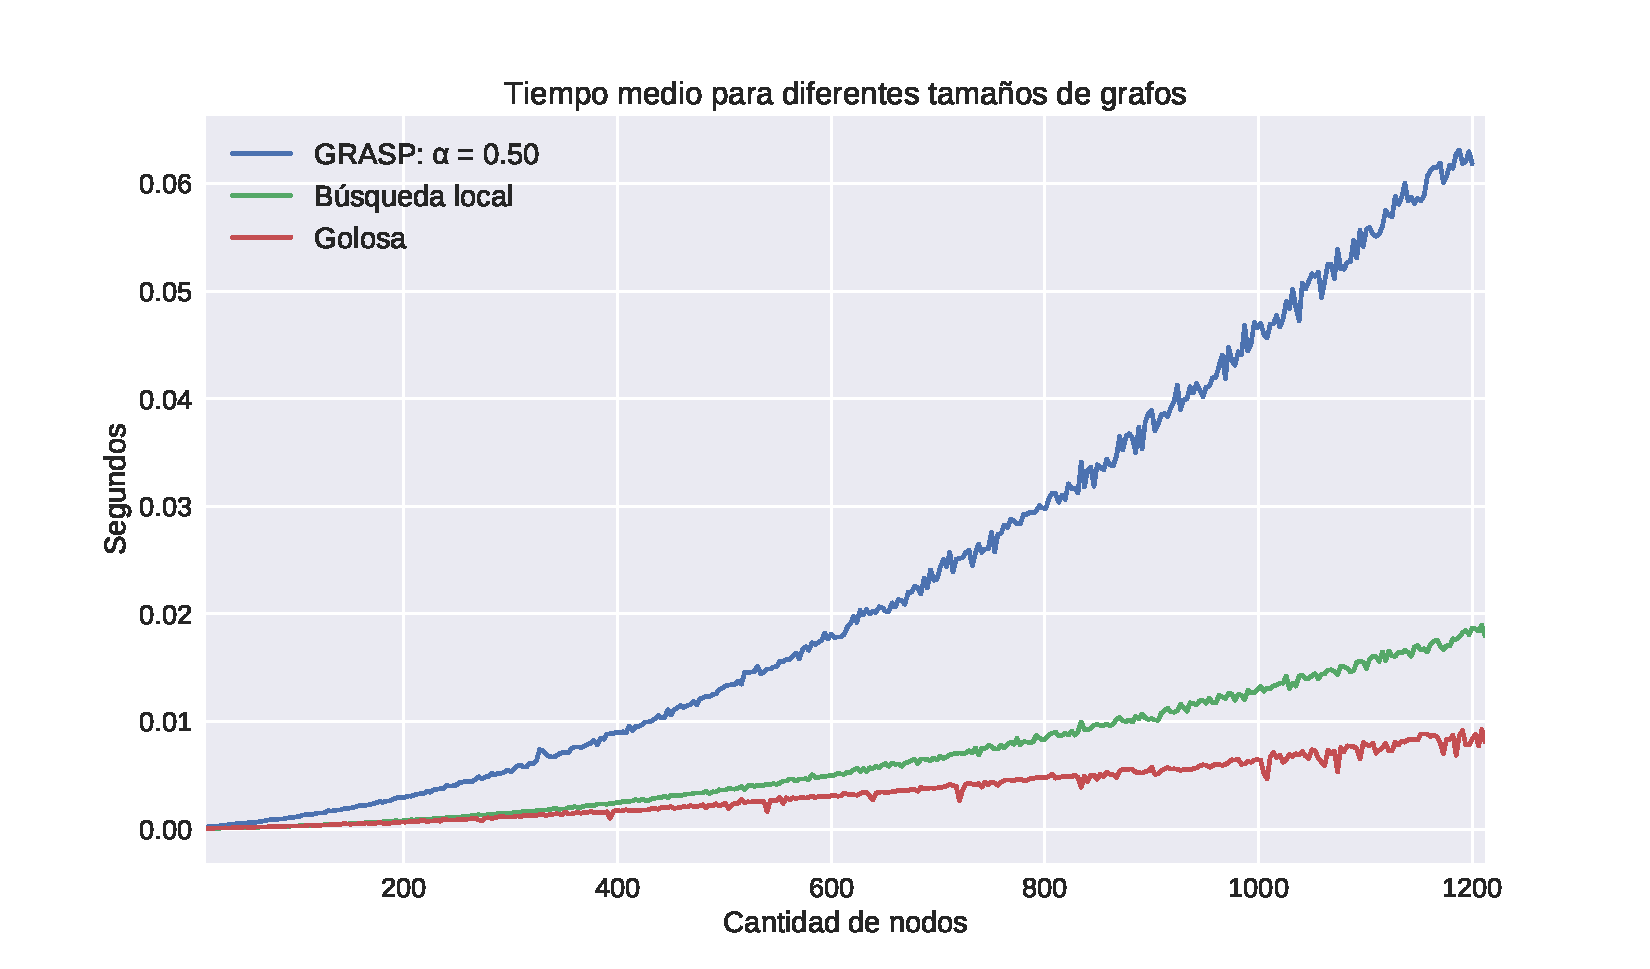
\includegraphics[width=1\textwidth]{informe/imgs/exp_malo_tiempo_grasp_local_greedy.pdf}
% }
El nivel de aleatoriedad con el que se crea la RCL del GRASP depende de nuestro parámetro $\alpha$. $\alpha = 0$ representa una elección puramente greedy, mientras que $\alpha = 1$ hace una elección puramente aleatoria. Dado nuestros grafos son bastantes particulares, al introducir un poco de aleatoriedad con el alpha ya logramos obtener las mejores fronteras posibles. Puede verse que, como adelantamos, cuando alpha es 0 se produce una elección puramente greedy, por lo que siempre es peor. \\

Es importante aclarar que esto es así por el tipo particular de grafos que estamos tratando, en el caso general esto puede no ser cierto. Intuitivamente los mejores resultados se obtienen en el equilibrio, con $\alpha = $0.5, por lo que en los siguientes casos utilizaremos este valor. \\

\todo[inline]{¿Qué es este gráfico?}

{\centering
    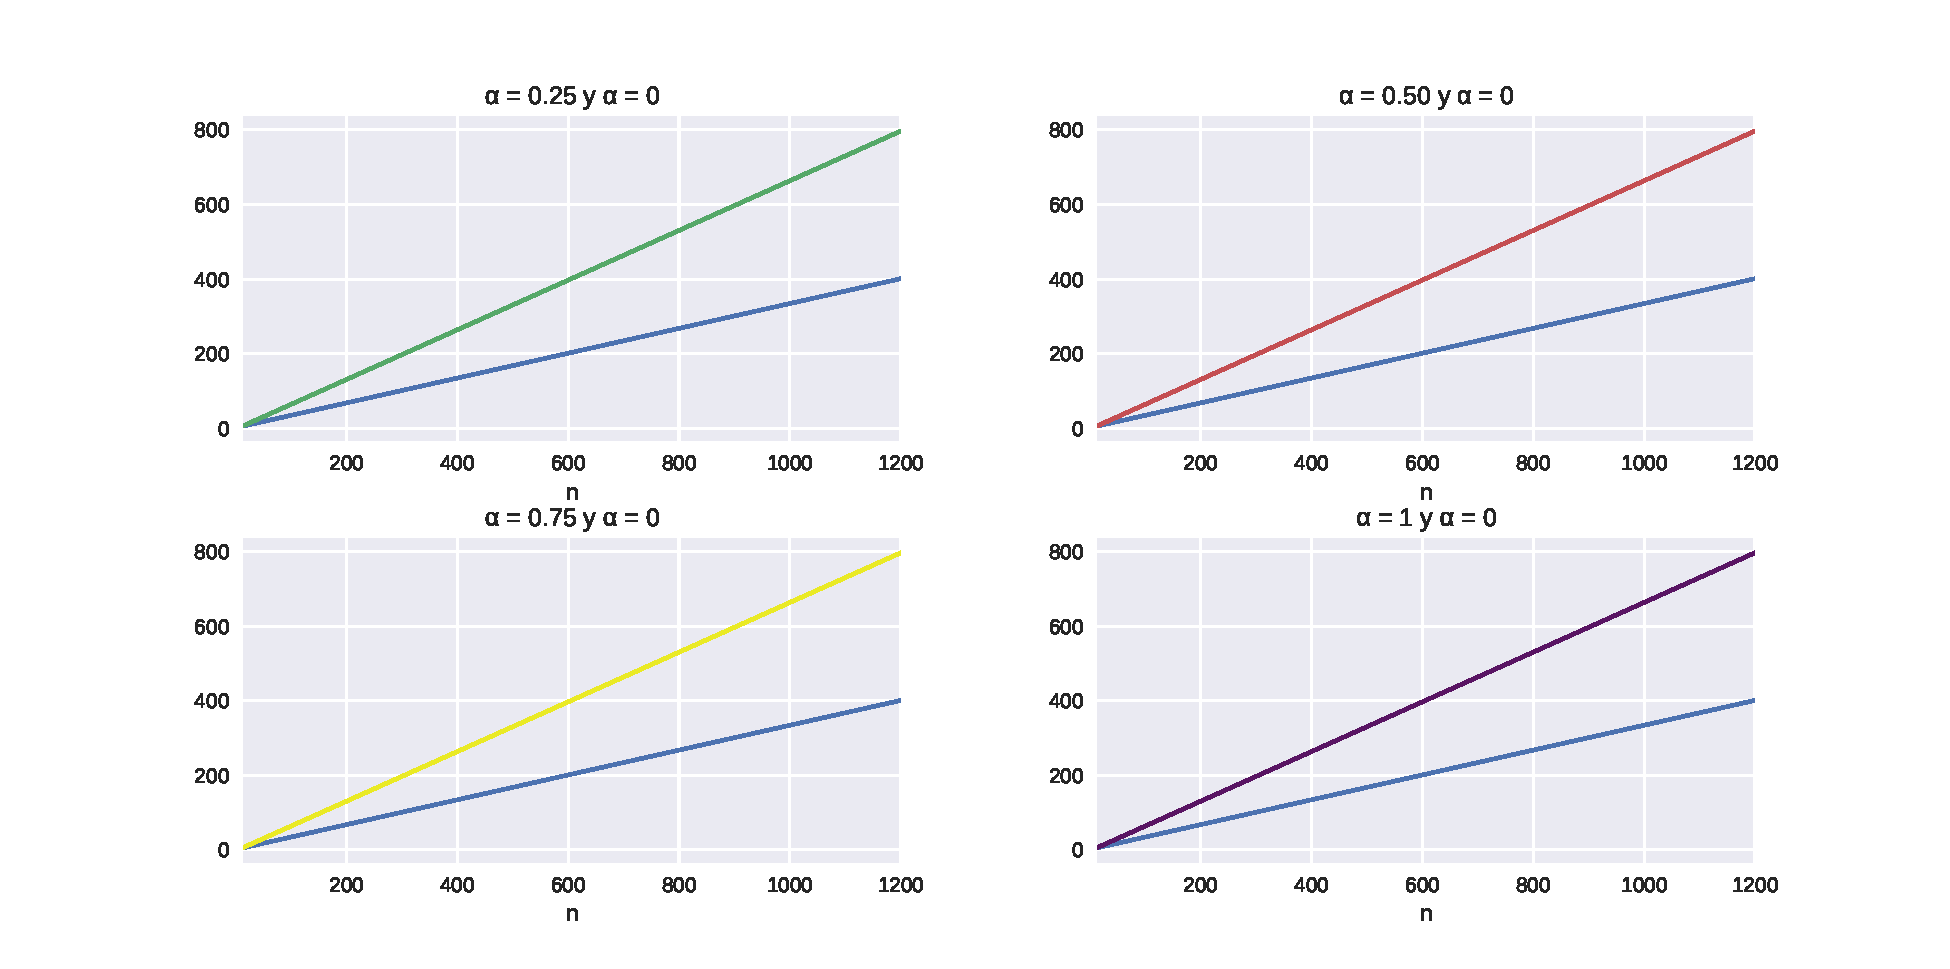
\includegraphics[width=1\textwidth]{informe/imgs/exp_malo_frontera_grasp_alphas.pdf}
}

% Esto era fruta completamente, tenia que ver con que se hacian muy pocas iteraciones de grasp y local
% {\centering
%     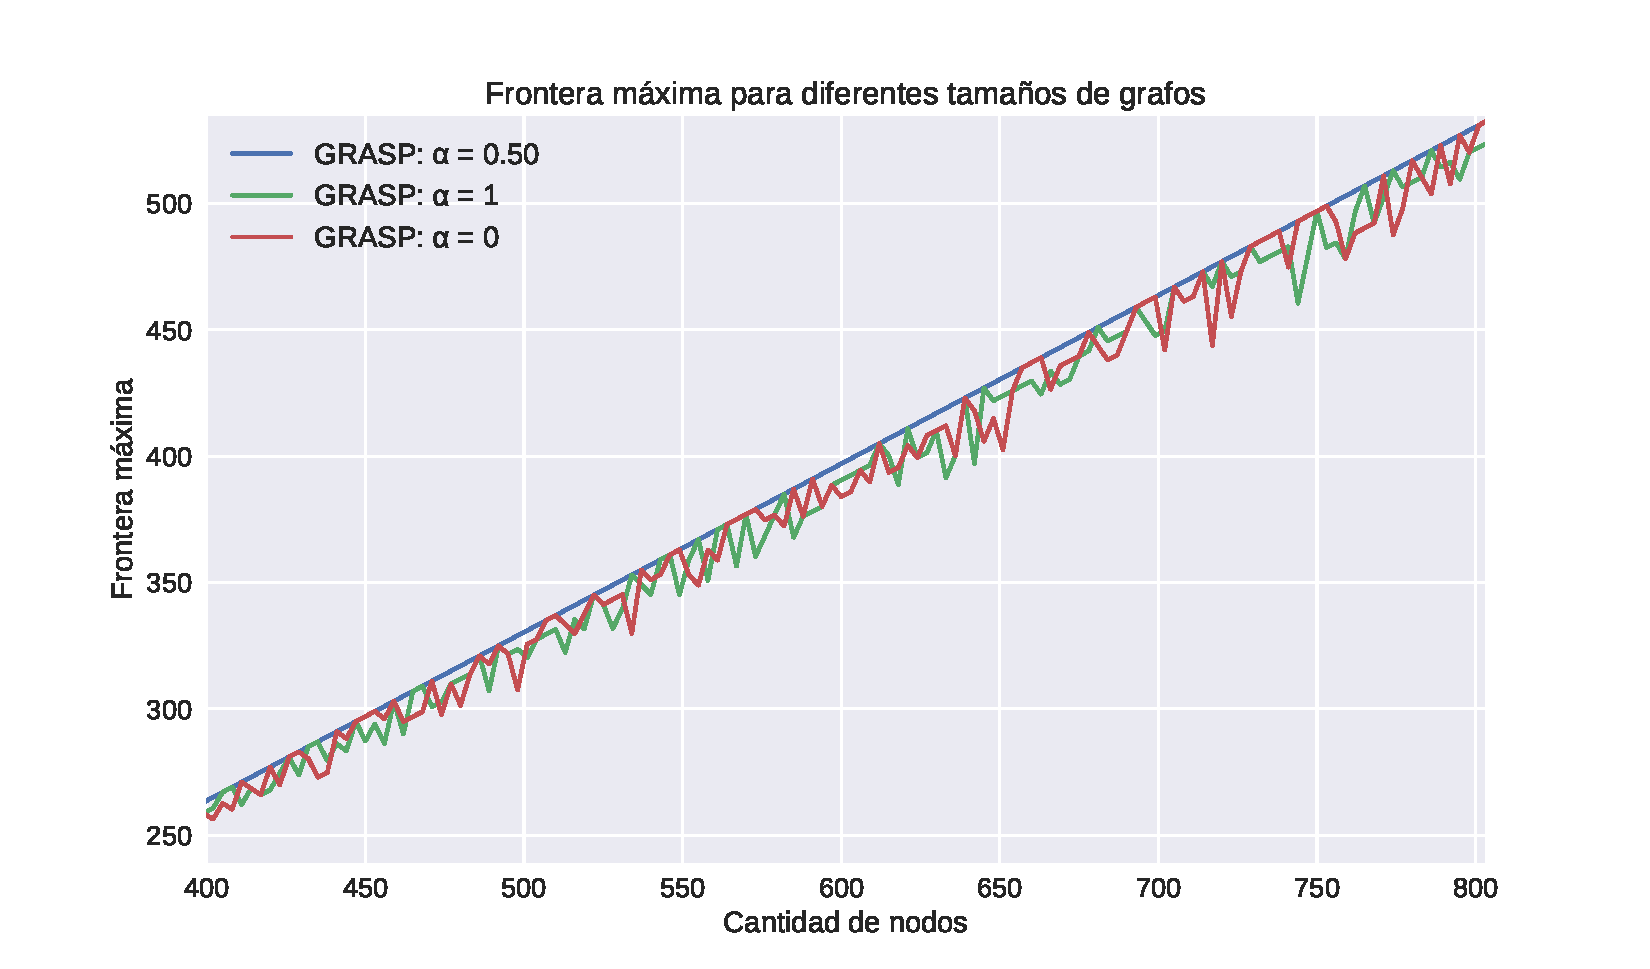
\includegraphics[width=0.90\textwidth]{informe/imgs/exp_malo_frontera_grasp_zoom.pdf}
%     % \captionof{figure}{$\uparrow$ Zoom del gráfico anterior}
% }

Otro parámetro importante es la cantidad de iteraciones a realizar, tanto en GRASP como en la búsqueda local interna. Para búsqueda local utilizamos $repsLocal = 2000$, al igual que en el apartado anterior. Con $repsGrasp$ fuimos variándolo y no encontramos ninguna diferencia apreciable, creemos que es por el tipo de grafo. Para estos experimentos tomamos $repsGrasp = 50$. \\

Nos interesa averiguar entonces qué tan lejos estamos del óptimo para nuestros ``grafos malos''. Estamos interesados en saber si la estrategia para escapar de los extremos locales funciona. Veamos lo que nos muestran los datos, recordando que anteriormente pudimos calcular cuál es la solución óptima para este tipo de grafos. \\

{\centering
    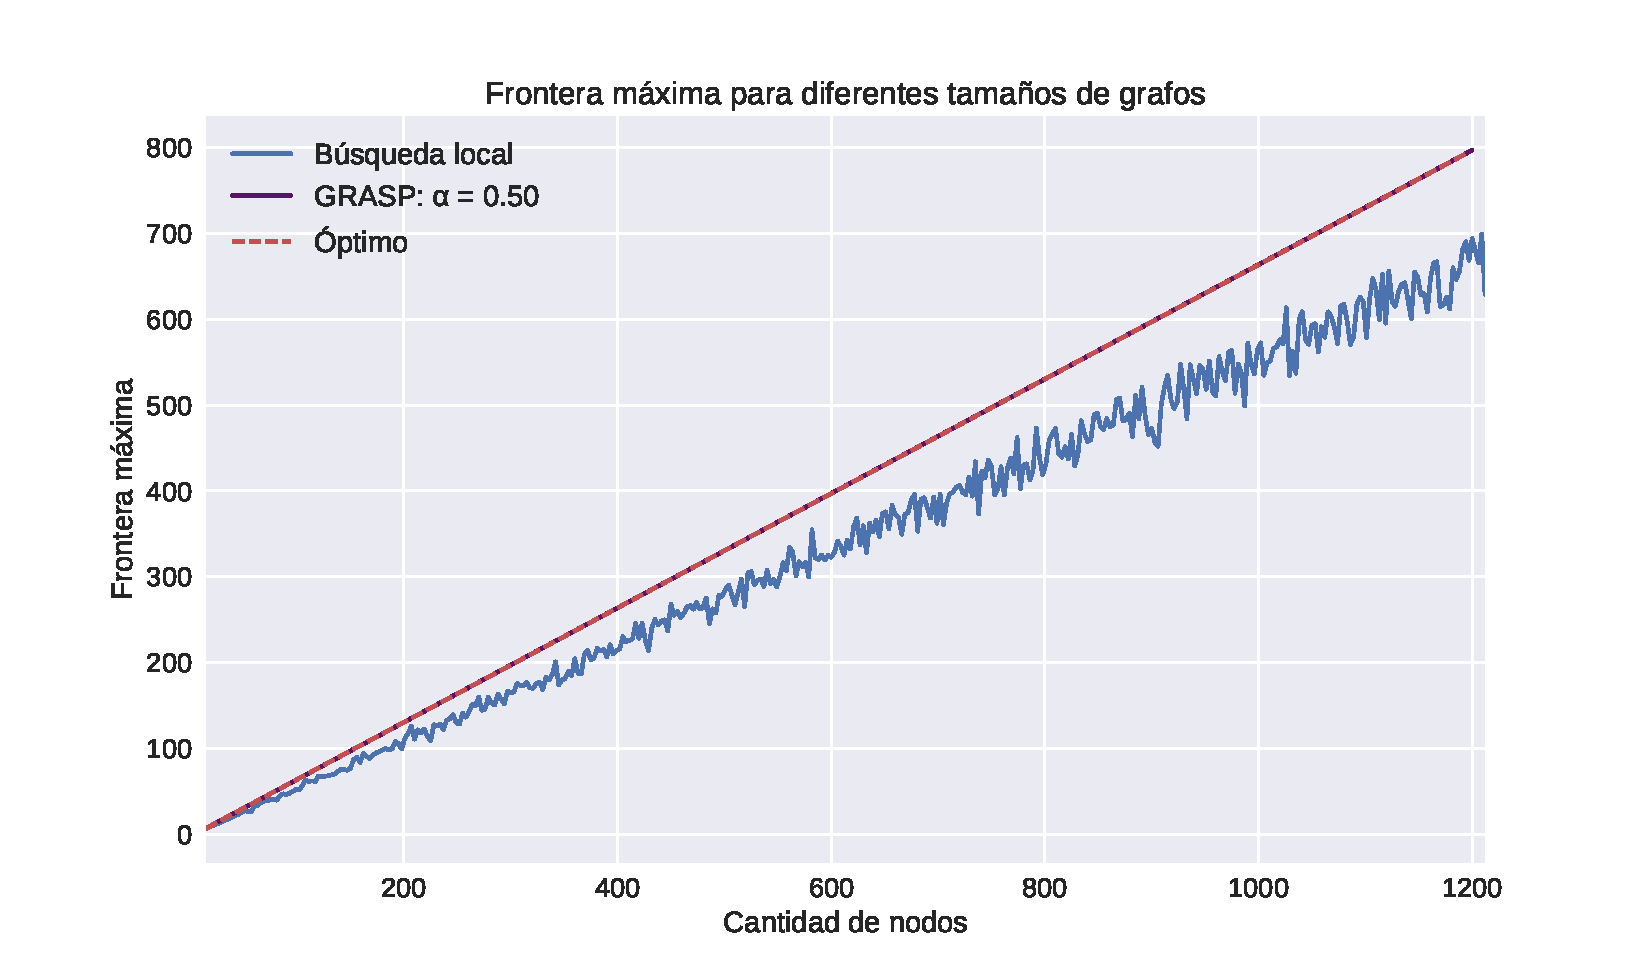
\includegraphics[width=1\textwidth]{informe/imgs/exp_malo_frontera_grasp_local_optimo.pdf}
}

¡La solución promedio de GRASP es \textbf{exactamente} la solución óptima! \\

Logramos resolver el problema de forma óptima para el caso en los que las demas técnicas fallaban. Es esperable que GRASP también sea bastante bueno para grafos en general. Veremos qué tan cierta es esta intuición en la siguiente sección. \\

Antes de concluir con este apartado, es interesante considerar cuál es el costo temporal de utilizar GRASP dependiendo el valor de $\alpha$. Aquí unas comparaciones:

{\centering
    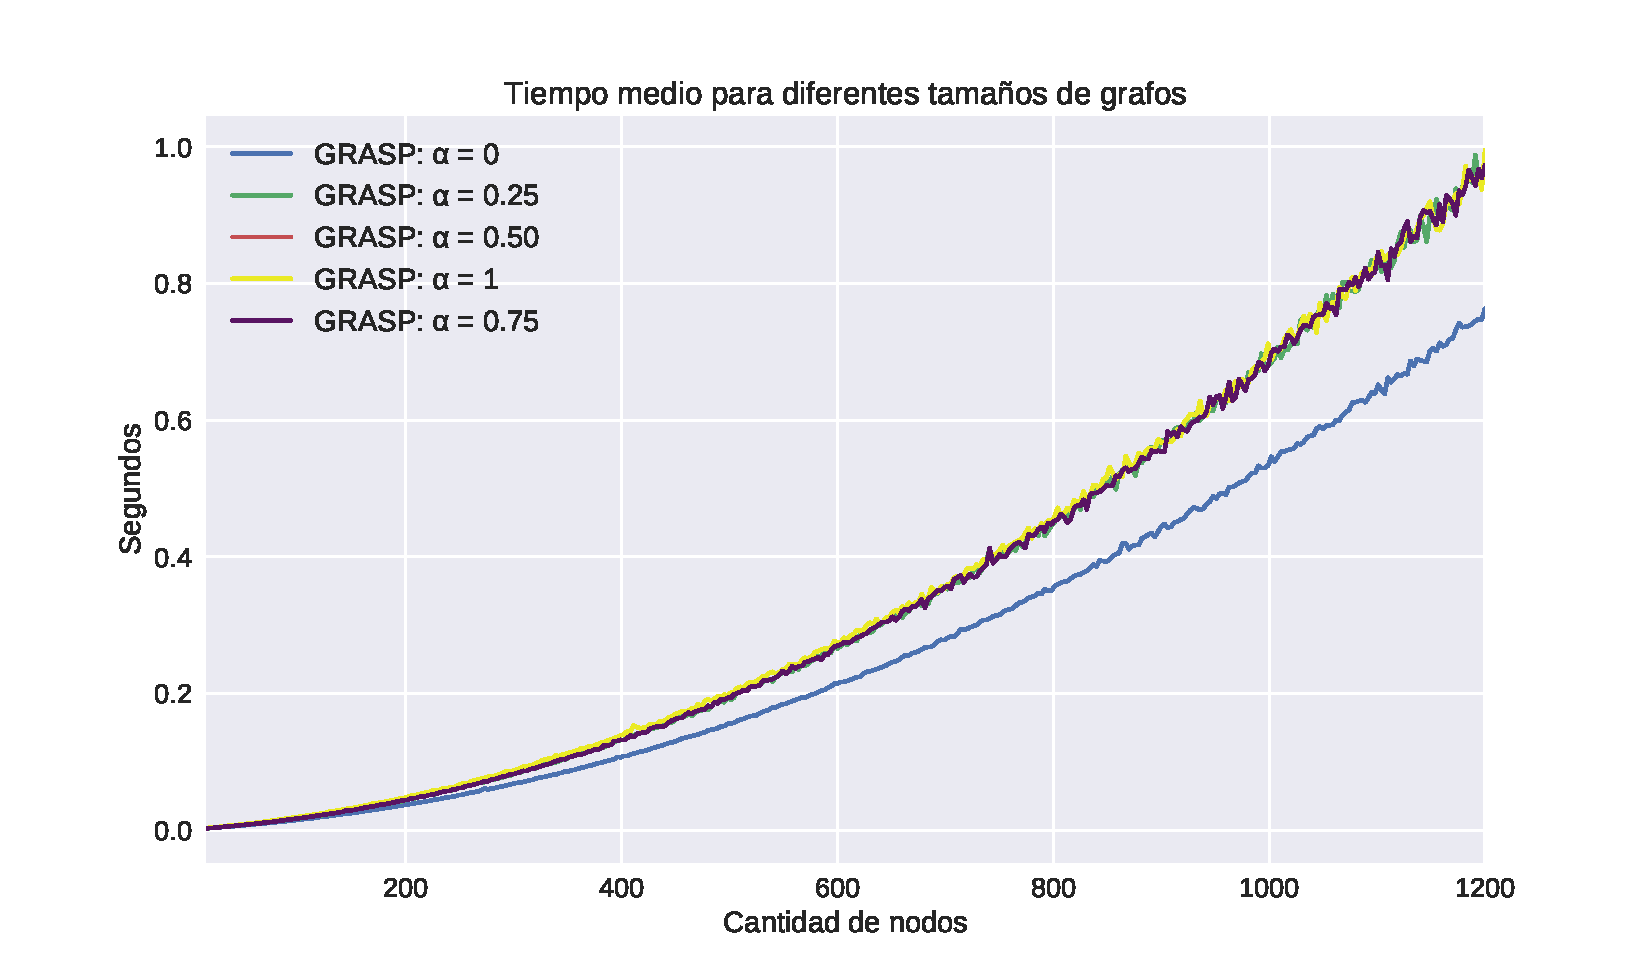
\includegraphics[width=1\textwidth]{informe/imgs/exp_malo_tiempo_grasp.pdf}
}


\newpage
% !TEX root = ./informe.tex
\section{Experimentación general}

Dado que nuestros análisis estaban enfocados en los peores casos, es momento de considerar cómo son nuestras soluciones si consideramos casos promedios.  \\

Consideramos que un grafo de $n$ nodos es promedio cuando generamos sus aristas al azar. Esto significa que las conexiones entre nodos será aleatoria, pero que la cantidad de aristas estará predeterminada con algun porcentaje, para poder separar mejor los diferentes casos de análisis. En particular, mostraremos los casos donde hay 50\% y 75\% de aristas. Demás porcentajes resultaron muy poco interesantes por tener muy pocas aristas o demasiadas. Como última aclaración, para todas las instancias de búsqueda local, la cantidad de repeticiones usadas es $2000$, a menos que se mencione explícitamente. \\

Nuestra intención es comparar exactamente qué tan mejores o peores son los diferentes algoritmos utilizados. Para esto, para cada tamaño de $n$ generamos un grafo al azar (con cierto porcentaje de aristas) y comparamos las soluciones obtenidas por todas las técnicas. Lo que sigue no son promedios, sino las soluciones finales para algun caso aleatorio dado. \\

{\centering
    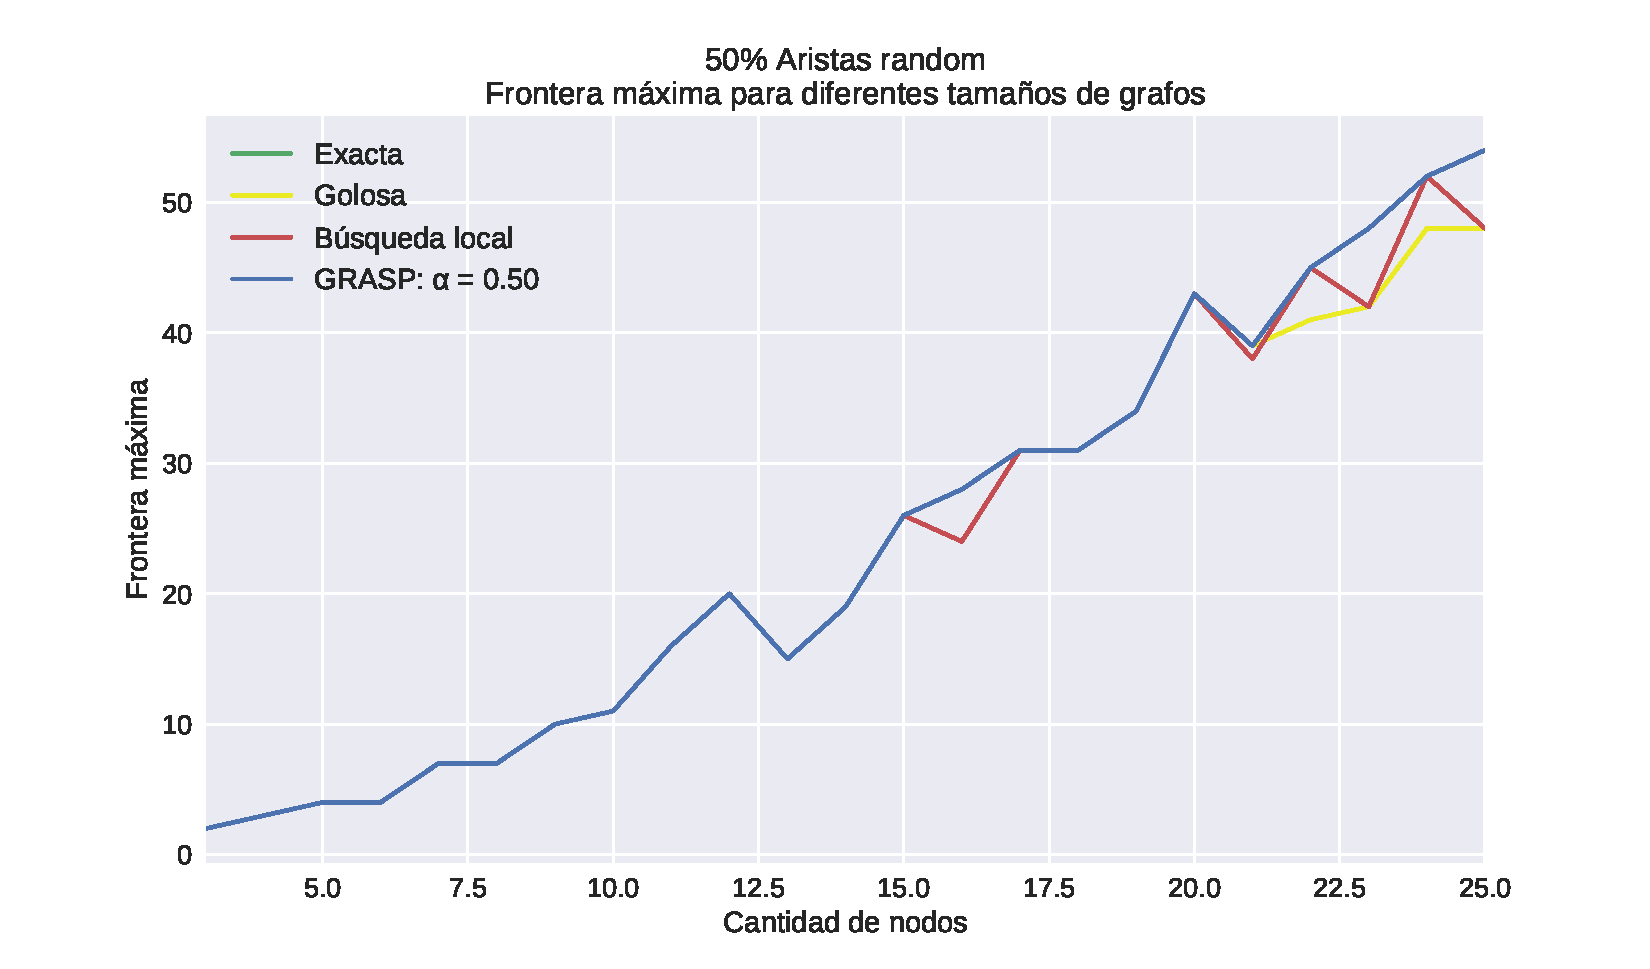
\includegraphics[width=0.9\textwidth]{informe/imgs/exp_random50_frontera_todos_v2.pdf}
    \captionof{figure}{$\uparrow$ Exacta y GRASP comparten la misma curva}
}
$ $ \newline

Los resultados son los que nuestros análisis anteriores apuntaban. Debemos tener en cuenta que son valores de $n$ pequeños (para poder comparar con el algoritmo exacto), veremos más adelante comparaciones para $n$ mayores. \\

Observamos que GRASP es la mejor técnica de las presentadas para resolver el problema. De hecho, comparte la misma curva que el algoritmo exacto. Le siguen el algoritmo de búsqueda local, y por último el goloso. Como sospechábamos, si bien en el análisis para un ``grafo malo'' el greedy era extremadamente malo, aquí podemos notar que para grafos en general conseguimos una aproximación bastante buena. \\

Analicemos tambíen que pasa con los tiempos de cómputo. Como era esperable, el tiempo del algoritmo exacto crece muy rápidamente, así que mostramos el gráfico en \textit{escala logarítmica}. En general son tiempos esperados, pero es interesante notar que GRASP tiene una constante asociada mucho mas elevada que los demás. \\

{\centering
    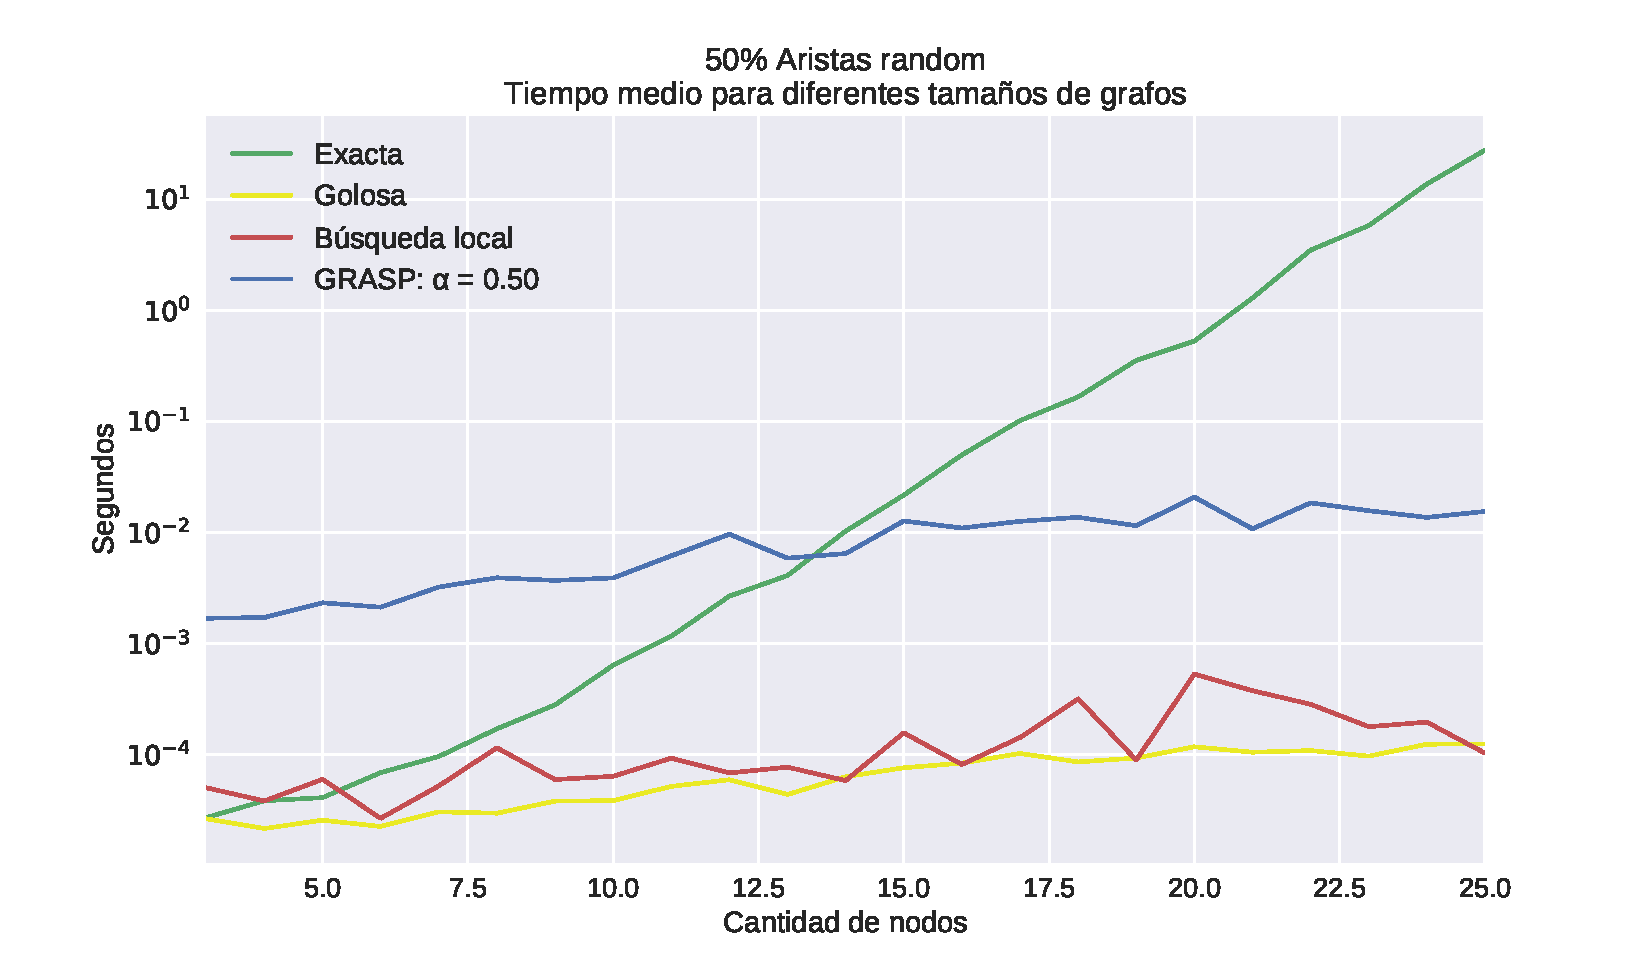
\includegraphics[width=0.9\textwidth]{informe/imgs/exp_random50_tiempo_todos_v2.pdf}
    \captionof{figure}{$\uparrow$ Escala logarítmica}
}
$ $ \newline

Repetimos el experimento pero para grafos con 75\% de aristas. Sin embargo, todos los algoritmos nos dan la misma solución (¡La óptima!). Esto tiene que ver con la densidad del grafo, y probablemente porque estamos viendo tamaños pequeños. \\

{\centering
    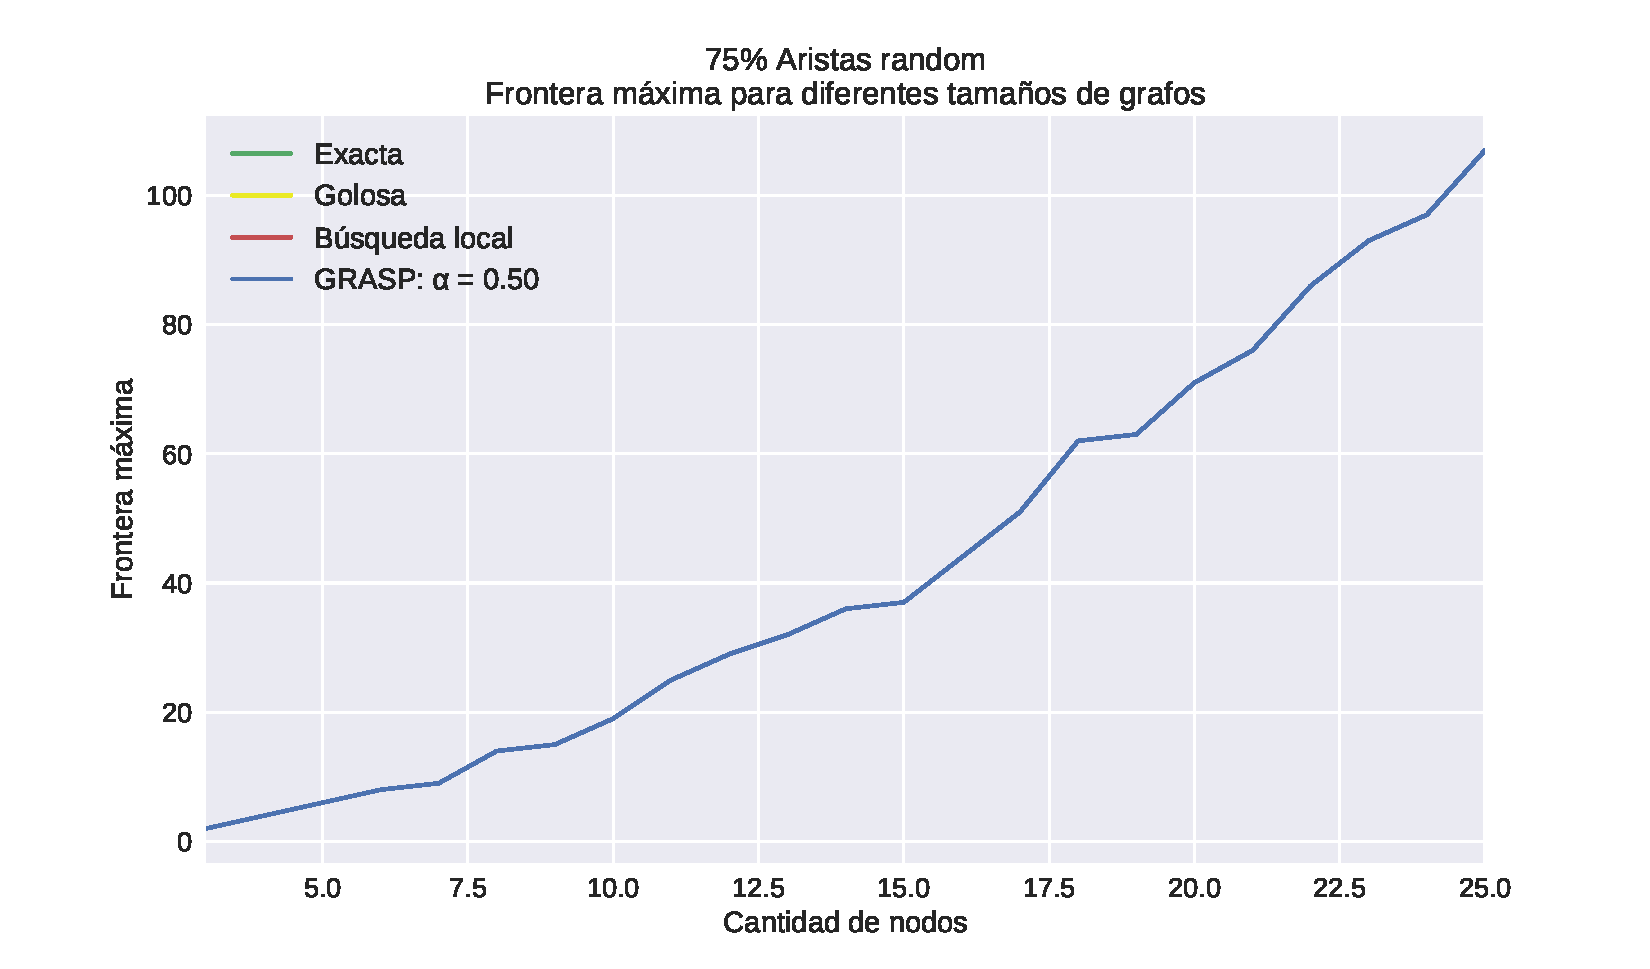
\includegraphics[width=0.9\textwidth]{informe/imgs/exp_random75_frontera_todos_v2.pdf}

}
$ $ \newline

Veamos que sucede si hacemos crecer $n$. Dado que no podemos realizar las pruebas para el algoritmo exacto debido a su complejidad temporal, no lo incluimos en el gráfico. No tenemos ninguna certeza de cuán cerca o lejos están de la solución óptima, pero es interesante observar como varían las diferentes soluciones. No incluímos 75\% aristas pues es idéntico al de 50\%. \\

{\centering
    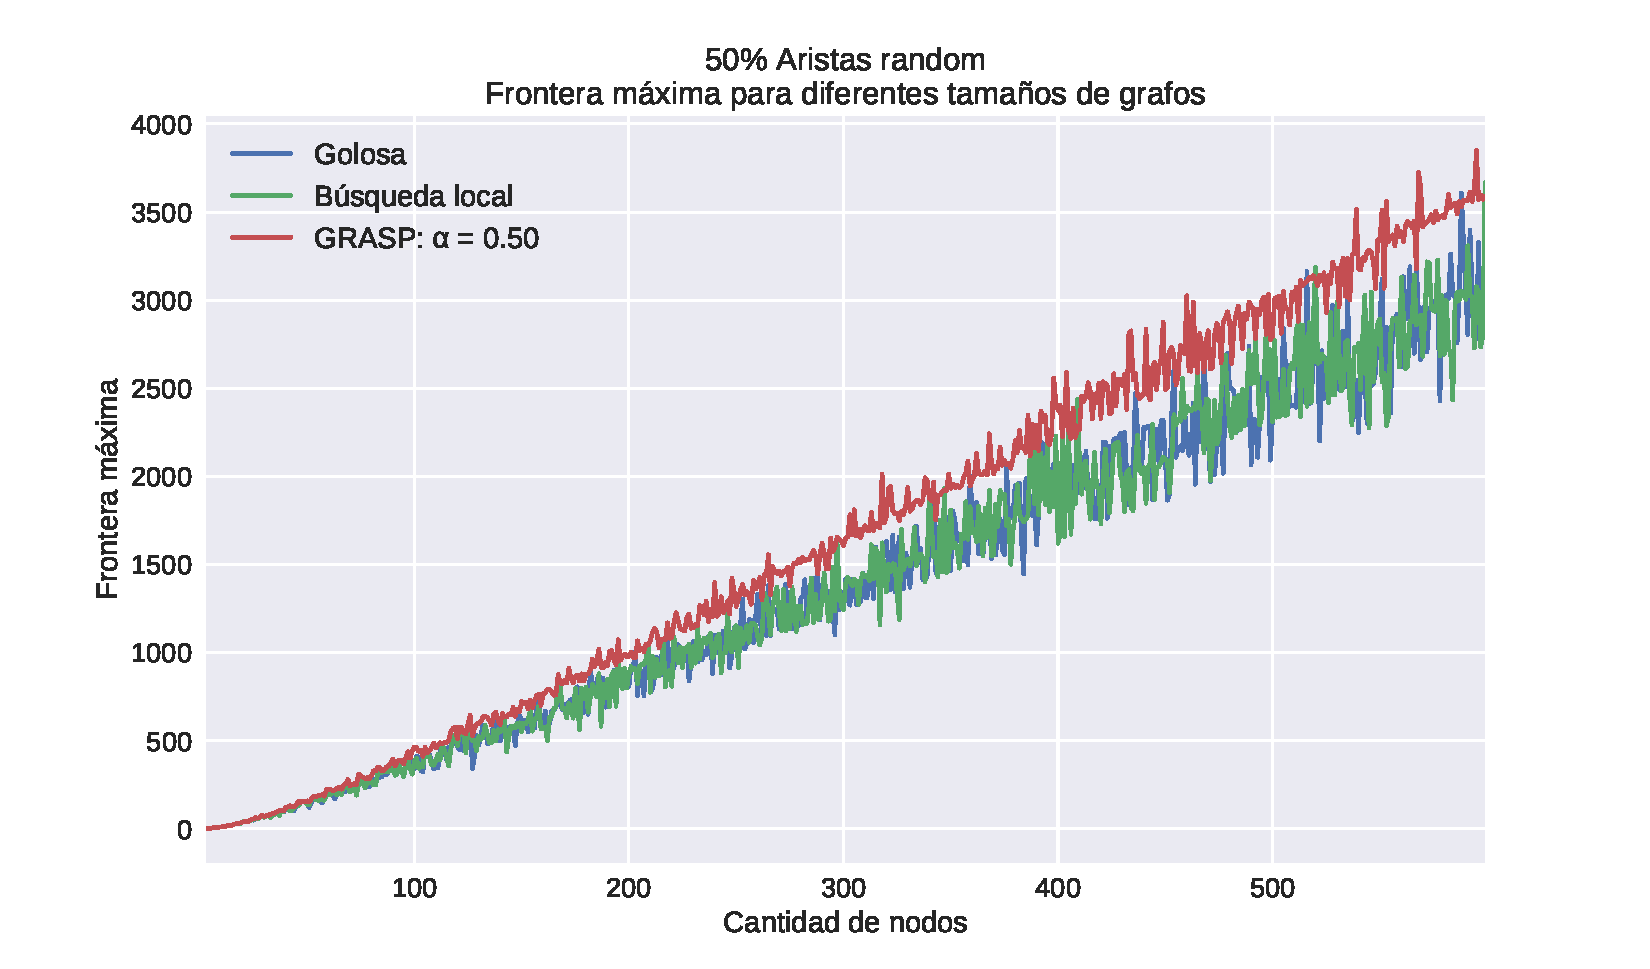
\includegraphics[width=0.9\textwidth]{informe/imgs/exp_random50_frontera_todos_ngrande.pdf}

}
$ $ \newline

Como esperábamos, GRASP es la mejor alternativa que tenemos para resolver el problema de CMF. El componente random sumado a la cantidad de repeticiones hacen que sea superior a los demás algoritmos, en términos de aproximación a la solución óptima. Variando la cantidad de $repsGrasp$ no obtuvimos diferencias significativas. En el gráfico se muestra con $repsGrasp = 50$. \\

GRASP es mejor, ¿pero a qué costo? Mostramos el gráfico en \textit{escala logárítmica} debido al tamaño de los tiempos de GRASP en comparación a los demás. Podemos observar claramente que el costo temporal es incluso mayor al esperado, dónde para $n = 600$ se demora aproximadamente 3 segundos. Esto entra en linea con la constante que habiamos observado en el anterior gráfico de tiempos. Es más que razonable, ya que estamos repitiendo dos algoritmos $O(n^5)$ en este caso $50$ veces. \\

{\centering
    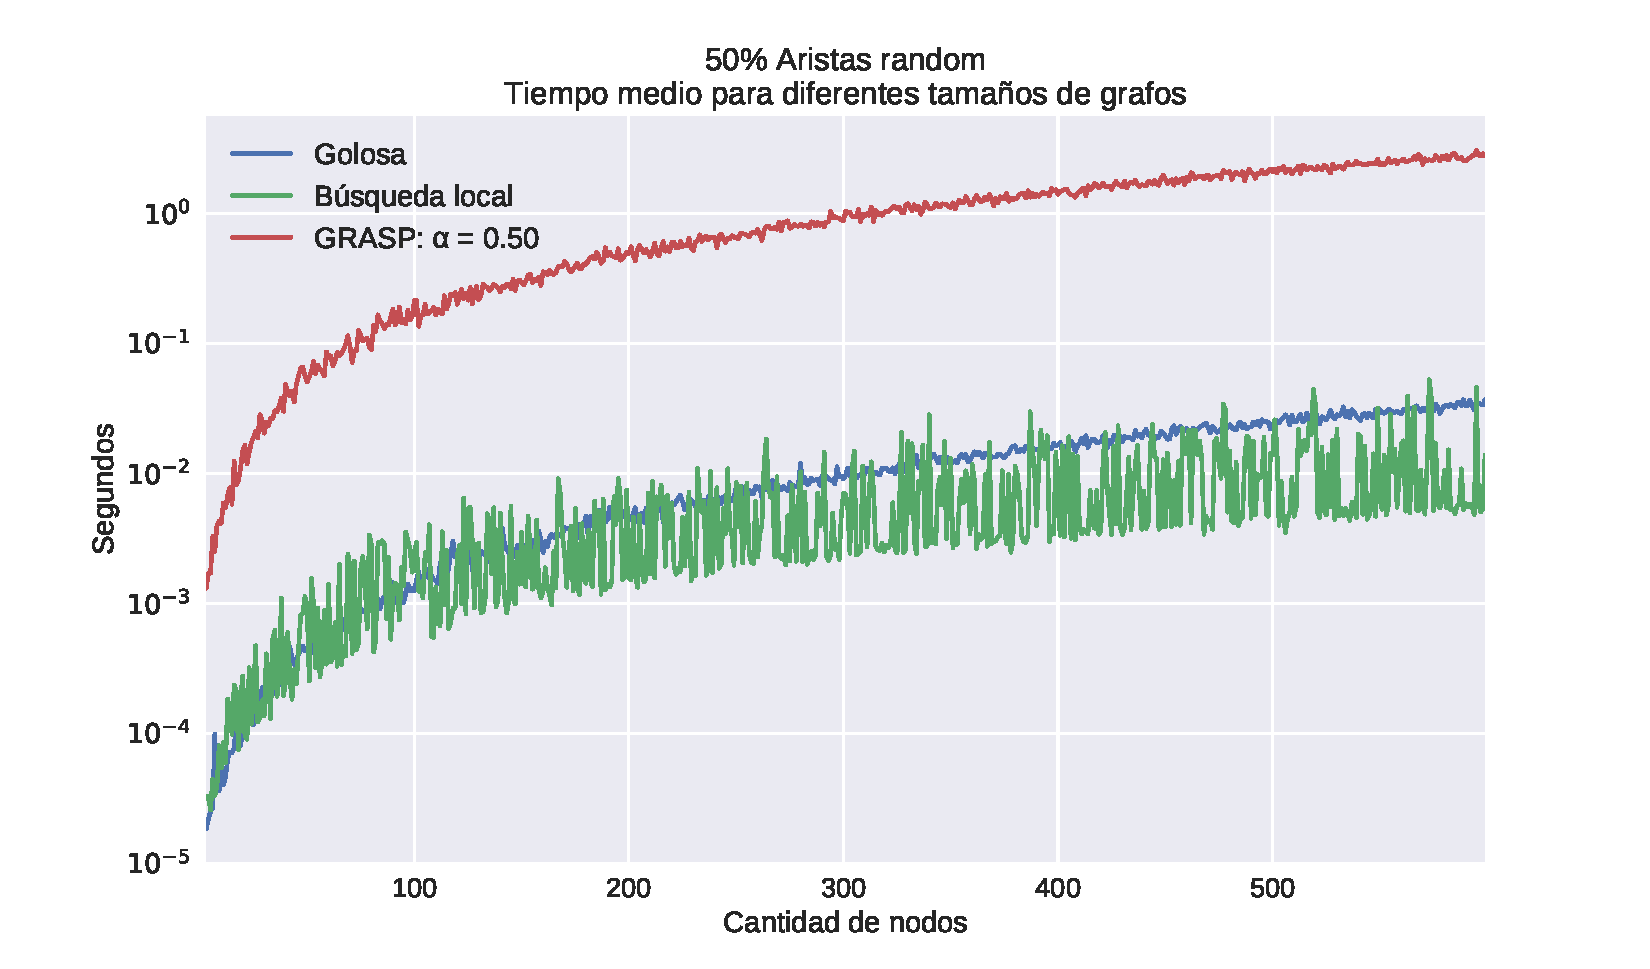
\includegraphics[width=0.9\textwidth]{informe/imgs/exp_random50_tiempo_todos_ngrande_logy.pdf}

}
$ $ \newline

El caso de tiempos de 75\% aristas no lo mostramos por ser idéntico en forma al anterior, pero en ese caso, con $n = 600$, GRASP tarda aproximadamente 17 segundos. Pueden disminuirse la cantidad de iteraciones para obtener una mayor eficiencia en términos del tiempo, pero a medida que $n$ crece GRASP es el primero que se vuelve inutilizable.

% No vale la pena por ser igual a 50%
% {\centering
%     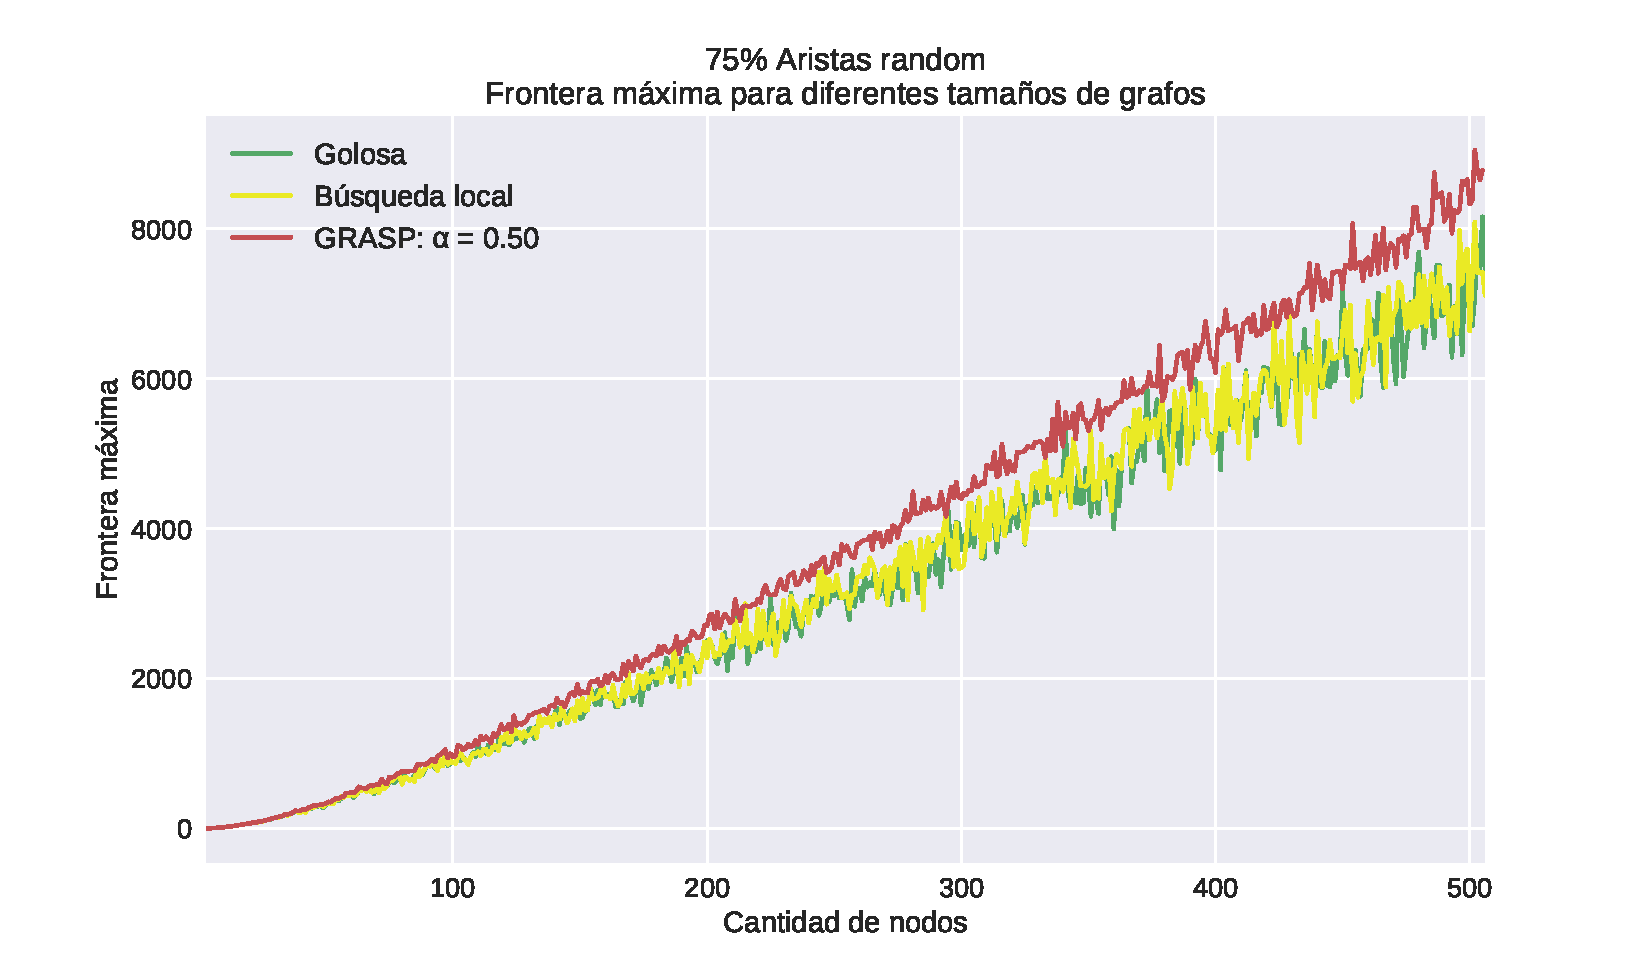
\includegraphics[width=1\textwidth]{informe/imgs/exp_random75_frontera_todos_ngrande.pdf}
% }


\subsection{Conclusión}

El objetivo de este trabajo era la investigación de diferentes técnicas para resolver el problema de Clique de Máxima Frontera. Sabemos que no se conoce hasta el momento ningún algoritmo exacto que lo resuelva en tiempo polinomial, por lo que mostramos una única forma de resolverlo de forma exacta, con complejidad temporal exponencial. \\

Vimos que el algoritmo exacto es inutilizable en la práctica para grafos con mas de 30 nodos, así que en la práctica es necesario recurrir a heurísticas que resuelvan el problema. \\

Consideramos un algoritmo sencillo, \textbf{greedy}, para intentar conseguir una buena solución. Lo que logramos encontrar fue un algoritmo exponencialmente mas rápido que en general da aproximaciones razonables. Encontramos además, al menos un tipo particular de grafos, los ``grafos malos'', para los cuales demostramos que la diferencia entre la solución óptima y la solución greedy tendía a infinito. \\

Intentando ahora poder solucionar el problema de ``grafos malos'', consideramos una heurística de \textbf{búsqueda local} para mejorar soluciones preexistentes, en dónde analizamos distintas formas de movernos a soluciones similares. Si bien en ocasiones logramos mejorar el método anterior, seguimos cayendo en el problema de que una vez llegados a un extremo local ya nos era imposible salir de ahí pues ninguna solución en su vecindad la mejoraría. \\

Para finalizar, nos basamos en el paper citado \cite{paper_grasp} para construir una solución que use el método GRASP. Con la introducción de variables aleatorias en conjunto con cierta estrategia golosa, logramos escapar del problema de los extremos locales pudiendo lograr así soluciones óptimas con gran probabilidad en nuestros grafos originales. \\

Una vez analizadas las distintas alternativas, probamos todos los algoritmos en una serie de grafos aleatorios, con diferentes porcentajes de aristas. Pudimos comprobar empíricamente lo analizado antes: GRASP produce los mejores resultados. Sin embargo, nos fue imposible dar una cota de distancia con respecto a la solución óptima porque no tenemos manera de conocer cuál es ésta solución sin poder correr el algoritmo exacto. \\


\newpage
% !TEX root = ../main.tex

\section{Bibliografía}

\begingroup
\renewcommand{\section}[2]{}% esto es pa sacar el Referencias

\begin{thebibliography}{}

\bibitem{proteins} Ina Koch, {\em Enumerating all connected maximal common subgraphs in
two graphs}

\end{thebibliography}

\end{document}
